\chapter{Soporte software del robot}
\label{cap:capitulo6}

\begin{flushright}
\begin{minipage}[]{10cm}
\emph{El software es una gran combinación entre arte e ingeniería}\\
\end{minipage}\\

Bill Gates\\
\end{flushright}

\vspace{1cm}
\setcounter{footnote}{72}

Una vez contado todo el proceso llevado a cabo para el diseño y construcción del prototipo robótico descrito, en este capítulo se explica la implementación \textit{software} desarrrollado para dar soporte a dicho prototipo.

\section{Simulación}
\label{sec:simulacion}

En esta sección se describe el proceso seguido para conseguir poner a PiBotJ en funcionamiento a través de simulación; en concreto, a través del simulador Gazebo. Esta parte ha sido desarrollada en el ordenador principal, explicado en la Sección \ref{subsec:ordenador}, apoyándose en el sistema ROS 2 Humble\footnote{\url{https://docs.ros.org/en/humble/Installation.html}}.

\subsection{URDF/Xacro}
\label{subsec:urdf}

Primero de todo fue necesario definir las estructuras y propiedades del robot. Para ello, se decidió usar el formato \ac{URDF}\footnote{\url{http://wiki.ros.org/urdf}} y \textit{Xacro}\footnote{\url{http://wiki.ros.org/xacro}}, muy comunes en aplicaciones robóticas. \acs{URDF} usa un formato de ficheros XML y describe al robot como un conjunto de \textit{links} (enlaces), que están conectadas por una serie de \textit{joints} (articulaciones); mientras que \textit{Xacro} usa también un formato de ficheros XML que permite crear URDF de manera más modular, reutilizable y eficiente mediante el uso de macros y propiedades\footnote{\url{https://articulatedrobotics.xyz/tutorials/ready-for-ros/urdf/}}.

En este proyecto se decidió crear una serie de ficheros \textit{Xacro}, cada uno dedicado a las distintas partes del robot (\verb|camera.xacro|\footnote{\url{https://github.com/RoboticsURJC/tfg-jlopez/blob/main/code/ros2/src/pibotj_r2c/description/camera.xacro}}, \verb|gps.xacro|\footnote{\url{https://github.com/RoboticsURJC/tfg-jlopez/blob/main/code/ros2/src/pibotj_r2c/description/gps.xacro}} y \verb|robot_core.xacro|\footnote{\url{https://github.com/RoboticsURJC/tfg-jlopez/blob/main/code/ros2/src/pibotj_r2c/description/robot_core.xacro}}). Cada fichero \textit{Xacro} necesita siempre tener la mismas etiquetas de \verb|<joint>| y \verb|<link>|, empleadas según convenga. Es importante usar herramientas como validadores de XML\footnote{\url{https://www.xmlvalidation.com/index.php?id=1&L=0\#xml-9-6--1732781305}} para evitar problemas.

Existen cuatro tipos de \textit{joint}: \textit{prismatic}, \textit{continuous}, \textit{revolute} y \textit{fixed}. En el Código \ref{cod:fj} se puede ver la definición de una \textit{fixed joint}; si se quiere usar otro tipo de \textit{joint}, hay que añadir algunos campos\footnote{\url{https://articulatedrobotics.xyz/tutorials/ready-for-ros/urdf/\#joint-tags}}.

\begin{code}[h]
	\begin{lstlisting}[language=xml]
		<joint name="gps_joint" type="fixed">
			<parent link="chassis"/>
			<child link="gps_frame"/>
			<origin xyz="-0.1 0.0 0.04" rpy="0 0 0"/>
		</joint>
	\end{lstlisting}
	\caption[Macro que define \textit{fixed joint}]{Macro que define una \textit{fixed joint}}
	\label{cod:fj}
			\end{code}

En relación a los \textit{link}\footnote{\url{https://articulatedrobotics.xyz/tutorials/ready-for-ros/urdf/\#link-tags}}, obligatoriamente tienen que tener las macros de \verb|<visual>|, \verb|<collision>| e \verb|<inertial>|, si no pueden surgir errores\footnote{\url{https://answers.gazebosim.org//question/25166/problem-changing-joint-from-fixed-to-revolute/}}. Existen cuatro tipos de geometría: \textit{box}, \textit{cylinder}, \textit{sphere} y \textit{mesh}. 
%El Código \ref{cod:ml} muestra un ejemplo de una \textit{mesh link}\footnote{\url{https://articulatedrobotics.xyz/tutorials/ready-for-ros/urdf/\#link-tags}}.

%\begin{code}[h]
%	\begin{lstlisting}[language=xml]
%		<link name="camera_link">
%			<visual>
%				<origin xyz="0.02 0.01 0.0 " rpy="0 0 ${-pi/2}"/>
%				<geometry>
%					<mesh filename="package://pibotj_r2c/meshes/camara.stl" scale="0.001 0.001 0.001"/>
%				</geometry>
%				<material name="Blue">
%					<color rgba="${0/255} ${0/255} ${255/255} 1.0"/>
%				</material>
%			</visual>
%			<collision> 
%				<origin xyz="0.0 0.0 0.0 " rpy="0 0 ${-pi/2}"/>
%				<geometry>
%					<mesh filename="package://pibotj_r2c/meshes/camara.stl" scale="0.001 0.001 0.001"/>
%				</geometry>
%			</collision>
%			<inertial>
%				<origin xyz="0.0 0.0 0.0" rpy="0 0 ${-pi/2}"/>
%				<mass value="0.03"/> <!--30g-->
%				<inertia ixx="0.01" ixy="0.0" ixz="0.0" iyy="0.005" iyz="0.0" izz="0.005"/>
%			</inertial>
%		</link>
%	\end{lstlisting}
%	\caption[Macro que define una \textit{mesh link}]{Macro que define una \textit{mesh link}}
%	\label{cod:ml}
%\end{code}


Una vez definidas las distintas partes del robot, se describen las interacciones del robot con el simulador; para ello se usa la macro \verb|<gazebo>|. En el presente proyecto, se ha simulado el sensor cámara y el módulo \acs{GPS}.Se pueden encontrar más ejemplos en la web oficial\footnote{\url{http://wiki.ros.org/urdf/XML/Gazebo}}.
%Existen muchos tipos de interacciones; en el Código \ref{cod:gazebo} se muestra; a modo de ejemplo, cómo simular el sensor cámara. Por su parte, para simular el módulo GPS se ha utilizado un mensaje del tipo NavSatFix\footnote{\url{http://docs.ros.org/en/api/sensor_msgs/html/msg/NavSatFix.html}}. Se pueden encontrar más ejemplos en la web oficial\footnote{\url{http://wiki.ros.org/urdf/XML/Gazebo}}.

%\begin{code}[h]
%	\begin{lstlisting}[language=xml]
%		<gazebo reference="camera_link_optical">
%		<material>Gazebo/Blue</material>
%			<sensor name="camera" type="camera">
%				<pose> 0 0 0 0 0 0 </pose>
%				<visualize>true</visualize>
%				<update_rate>10</update_rate>
%				<camera>
%					<horizontal_fov>1.089</horizontal_fov>
%					<image>
%						<format>R8G8B8</format>
%						<width>640</width>
%						<height>480</height>
%					</image>
%					<clip>
%						<near>0.05</near>
%						<far>8.0</far>
%					</clip>
%				</camera>
%				<plugin name="camera_controller" filename="libgazebo_ros_camera.so">
%					<frame_name>camera_link_optical</frame_name>
%				</plugin>
%			</sensor>
%		</gazebo>
%	\end{lstlisting}
%	\caption[Macro que permite a Gazebo simular una cámara]{Macro que permite a Gazebo simular una cámara}
%	\label{cod:gazebo}
%\end{code}

Asimismo, se han definido los sistemas de coordenadas que aparecen en la Figura \ref{fig:links}. Una vez se definió el robot y los sensores necesarios para que Gazebo interactuara con el modelo, se hizo uso de ROS 2 Control. 

\begin{figure} [h!]
	\begin{center}
		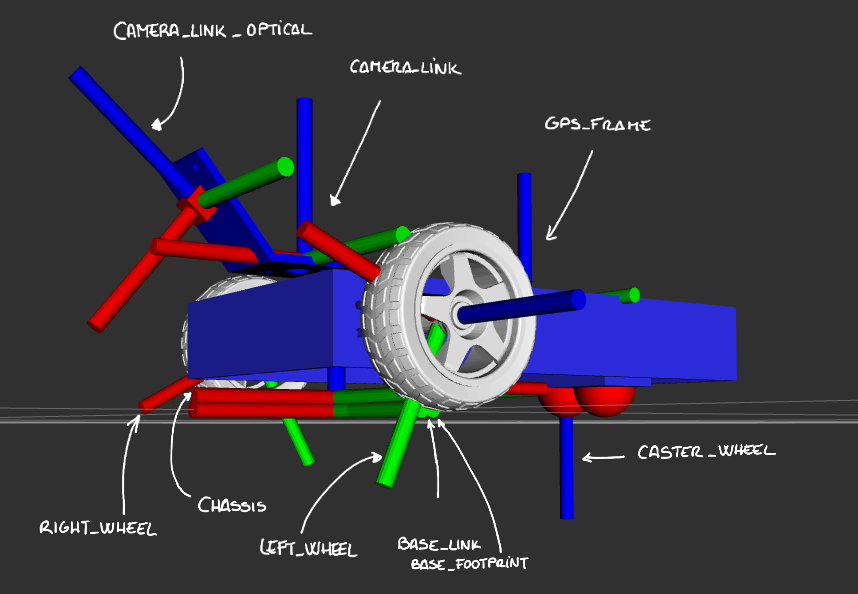
\includegraphics[width=13cm]{figs/cap6/links.png}
	\end{center}
	\caption{Sistemas de Coordenadas de PiBotJ}
	\label{fig:links}
\end{figure}


\subsection{ROS 2 Control}
\label{subsec:cap6ros2control}

Como se explicó en la Sección \ref{subsec:ros2control}, ROS 2 Control es un \textit{framework} que permite gestionar y controlar los sensores y actuadores de manera eficiente, y es por ello que se decidió aplicar a este proyecto a través del fichero \verb|ros2_control.xacro|\footnote{\url{https://github.com/RoboticsURJC/tfg-jlopez/blob/main/code/ros2/src/pibotj_r2c/description/ros2_control.xacro}}.

Para este proyecto se definió un sistema llamado \textit{GazeboSystem}, encargado del \textit{hardware interface}; de esta forma, es más sencillo añadir el número de sensores y actuadores que se necesiten. En muchos casos, se decidió controlar a \textit{left\_wheel\_joint}, \textit{right\_wheel\_joint} y a \textit{camera\_joint}, que son aquellos \textit{joints} que tenían asignados un motor en la vida real. 

Al ejecutar \verb|ros2 control list_hardware_interfaces| se puede ver las interfaces asociadas de lectura/escritura y de monitorización que tiene cada \textit{joint} a controlar. En la Figura \ref{fig:ros2control} se pueden ver las interfaces que tiene PiBotJ y, por ende, cómo se va a controlar cada interfaz.

 \begin{figure} [h!]
 	\begin{center}
 		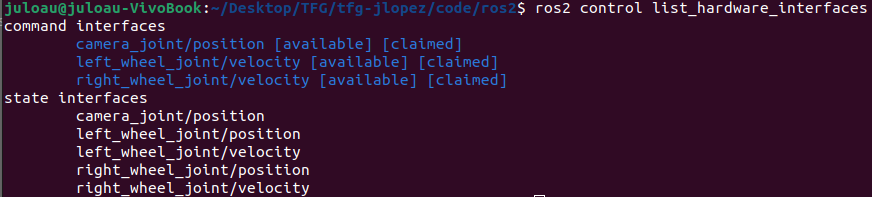
\includegraphics[width=14cm]{figs/cap6/interfaces.png}
 	\end{center}
 	\caption{Interfaces que tiene definidas PiBotJ}
 	\label{fig:ros2control}
 \end{figure}

Tras definir los \textit{joints} a controlar, era necesario definir en un fichero YAML el tipo de controladores que utilizaba el \textit{controller manager}. Dentro de cada controlador había que asignar los \textit{joints} definidos previamente al controlador que necesite cada una. En este caso, se asignaron las ruedas a un control diferencial y, la cámara, se decidió controlar por posición, usando el \textit{topic} \verb|\pos_cont|\footnote{\url{https://control.ros.org/humble/index.html}}.

Una vez el robot estaba completamente definido en los diferentes ficheros \textit{Xacro}, era necesario unirlos todos en otro fichero llamado \verb|robot.urdf.xacro|\footnote{\url{https://github.com/RoboticsURJC/tfg-jlopez/blob/main/code/ros2/src/pibotj_r2c/description/robot.urdf.xacro}} para poder facilitar la publicación del estado del robot, y eso se consigue usando \verb|robot_state_publisher|.
 
\subsection{Robot State Publisher}
\label{subsec:robotstatepublisher}

En la Web oficial de ROS\footnote{\url{http://wiki.ros.org/robot_state_publisher}} se explica que \verb|robot_state_publisher| es esencial para publicar las transformaciones (tf) entre los diferentes \textit{links} del robot y para proporcionar información sobre el estado de sus \textit{joints} a cualquier componente en el sistema. Aunque pueda parecer complicado, la Figura \ref{fig:rsp}, obtenida de la web de Articulated Robotics\footnote{\url{https://articulatedrobotics.xyz/tutorials/mobile-robot/concept-design/concept-urdf\#quick-recap}}, resume muy bien los pasos que sigue \verb|robot_state_publisher|.

 \begin{figure} [h!]
	\begin{center}
		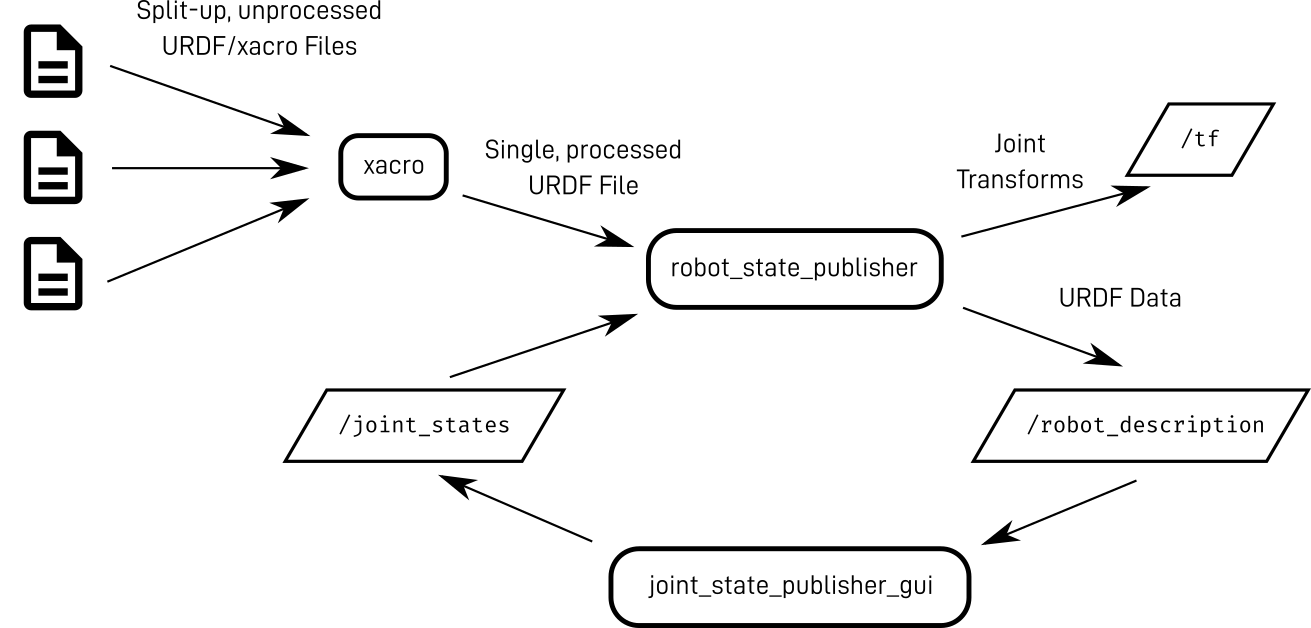
\includegraphics[width=12cm]{figs/cap6/rsp.png}
	\end{center}
	\caption{Diagrama de robot\_state\_publisher}
	\label{fig:rsp}
\end{figure}

Una vez todos los elementos a utilizar estaban listos, era el momento de aglutinarlos todos y crear un launcher que los inicializara y los pusiera en ejecución.

\subsection{Launcher}
\label{subsec:launcher}

El \textit{launcher} que se decidió crear para este proyecto parte del creado por Johnewans\footnote{\url{https://github.com/joshnewans/articubot_one/blob/main/launch/launch_sim.launch.py}}, creador de Articulated Robotics, y fue modificado según las necesidades, siendo finalmente el resultante \verb|launch_sim.launch.py|\footnote{\url{https://github.com/RoboticsURJC/tfg-jlopez/blob/main/code/ros2/src/pibotj_r2c/launch/launch_sim.launch.py}}. Para facilitar su entendimiento, la Figura \ref{fig:launcherdiagram} explica los componentes que forman parte del \textit{launcher}. Con esto, ya podemos ejecutar al completo el PiBotJ.


 \begin{figure} [h!]
	\begin{center}
		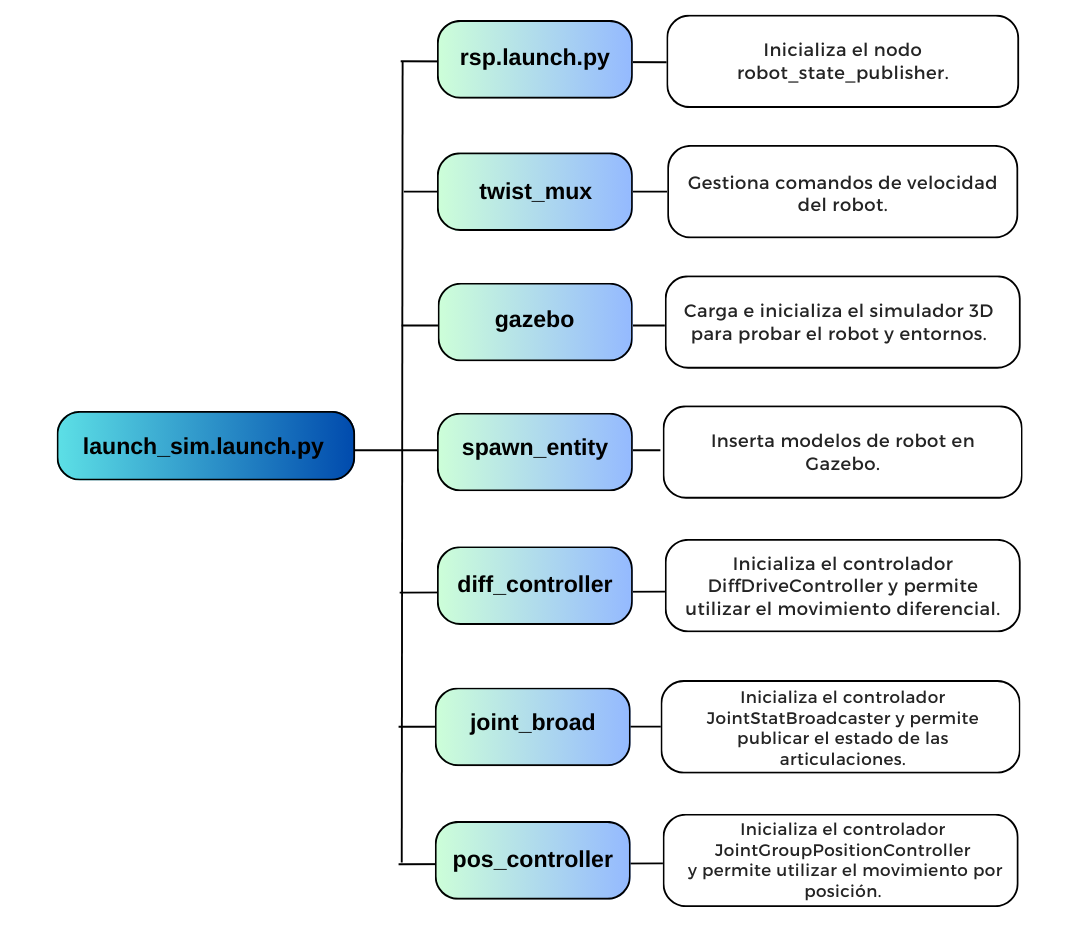
\includegraphics[width=14cm]{figs/cap6/diagram.png}
	\end{center}
	\caption{Esquema de launch\_sim.launch.py}
	\label{fig:launcherdiagram}
\end{figure}


\subsection{Ejecución en simulador}
\label{subsec:funsimulacion}

%Para mostrar todos los \textit{topics} que forman parte del robot, lanza el siguiente comando:  \verb|ros2 topic list|, y su salida se puede ver en la Figura \ref{fig:topic}.

La Figura \ref{fig:topic} muestra todos los \textit{topics} que forman parte del robot y para conseguir el objetivo propuesto en la Sección \ref{sec:descripcion}, es necesario utilizar únicamente: \verb|/camera/image_raw|, para ver la imagen de la cámara; \verb|/cmd_vel|, para mover las ruedas; \verb|/gps/data|, para ver los valores de posición del \acs{GPS}; y \verb|/pos_cont/commands|, para mover el motor de la cámara.

\begin{figure} [h!]
	\begin{center}
		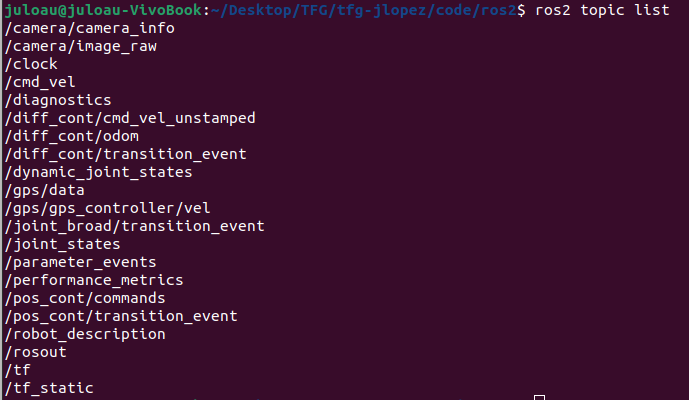
\includegraphics[width=12cm]{figs/cap6/topic.png}
	\end{center}
	\caption{Topics disponibles al lanzar el robot}
	\label{fig:topic}
\end{figure}


Para mover las ruedas hay muchas formas de hacerlo, pero en este caso se usó \verb|rqt_robot_steering|, como muestra la Figura \ref{fig:hercym} (izquierda). Si se quiere visualizar la cámara, se puede usar \verb|rviz2| o \verb|ros2 run rqt_image_view rqt_image_view|, que fue el comando usado para probar su funcionamiento (Figura \ref{fig:hercym} derecha). Por otro lado, los datos vertidos por el módulo \acs{GPS} se pueden visualizar usando \verb|ros2 topic echo /gps/data|, como muestra la Figura \ref{fig:echogps} y finalmente, para mover el motor de la cámara por posición, es necesario usar el comando siguiente: 

\begin{verbatim}
	ros2 topic pub /pos_cont/commands std_msgs/msg/Float64MultiArray \
	 "data: [-0.5]"
\end{verbatim} 

Siendo los valores que van dentro de \textit{data} desde 3 (giro hacia la izquierda) hasta -3 (giro hacia la derecha). 
%En la Figura \ref{fig:camararot} se pueden ver los dos casos descritos previamente. 


\begin{figure}[ht!]
	\centering
	\begin{minipage}{0.28\linewidth}
		\centering
		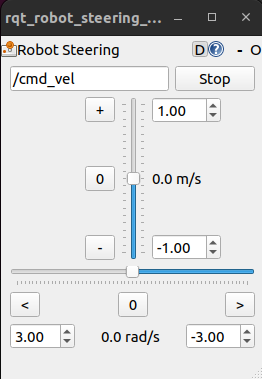
\includegraphics[width=\linewidth]{figs/cap6/steering.png}
		\caption*{\centering Mover las ruedas} 
	\end{minipage}
	\hspace{0.5 cm}
	\begin{minipage}{0.65\linewidth}
		\centering
		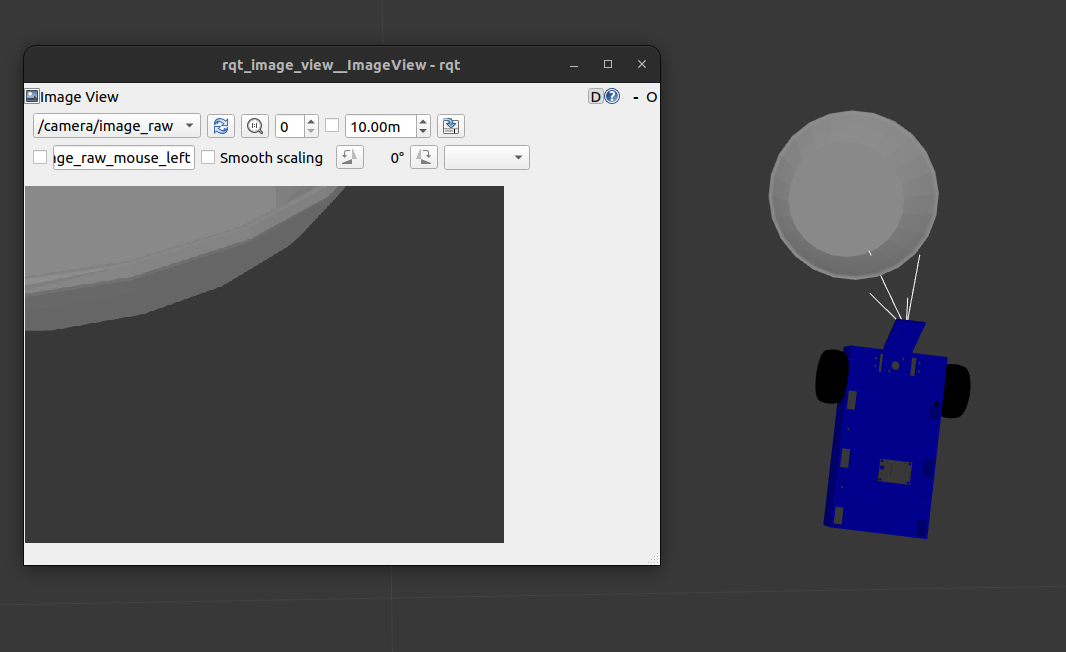
\includegraphics[width=\linewidth]{figs/cap6/rqtimage.png}
		\caption*{\centering Visualizar la cámara} 
	\end{minipage}
	\caption{Herramientas usadas}
	\label{fig:hercym}
\end{figure}

%\begin{figure} [h!]
%	\begin{center}
%		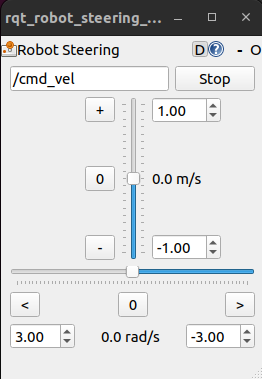
\includegraphics[width=6cm]{figs/cap6/steering.png}
%	\end{center}
%	\caption{Herramienta usada para mover las ruedas}
%	\label{fig:steering}
%\end{figure}

%\begin{figure} [h!]
%	\begin{center}
%		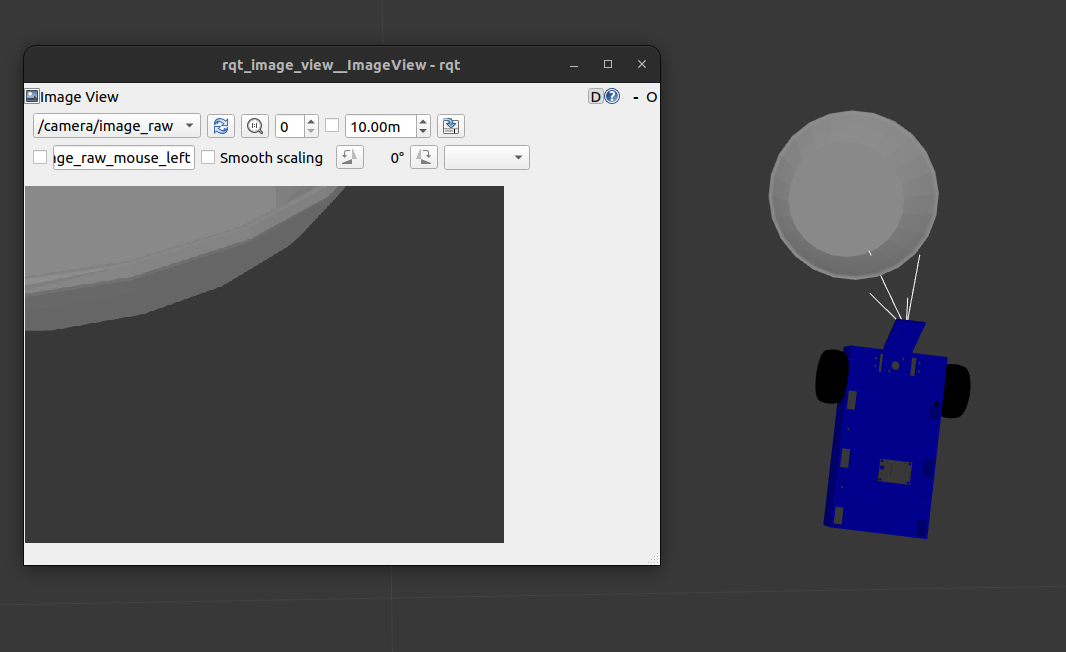
\includegraphics[width=12cm]{figs/cap6/rqtimage.png}
%	\end{center}
%	\caption{Herramienta usada para visualizar la cámara}
%	\label{fig:rqtimage}
%\end{figure}

 \begin{figure} [h!]
	\begin{center}
		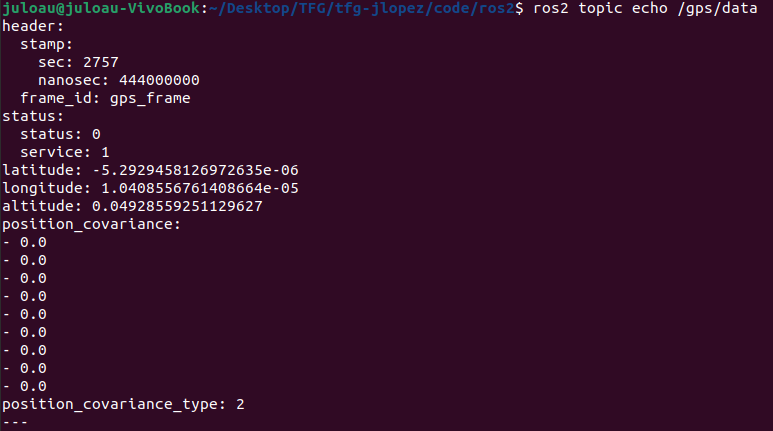
\includegraphics[width=11cm]{figs/cap6/echogps.png}
	\end{center}
	\caption{Herramienta usada para visualizar los valores del GPS}
	\label{fig:echogps}
\end{figure}


El resultado final, con el robot de PiBotJ funcionando en simulación, se puede apreciar en la secuencia mostrada en la Figura \ref{fig:camararot}, pudiéndose ver la ejecución completa en el vídeo\footnote{\url{https://www.youtube.com/watch?v=A0yi7YlLpq0}}. 

\begin{figure}[ht!]
	\centering
	\begin{minipage}{0.35\linewidth}
		\centering
		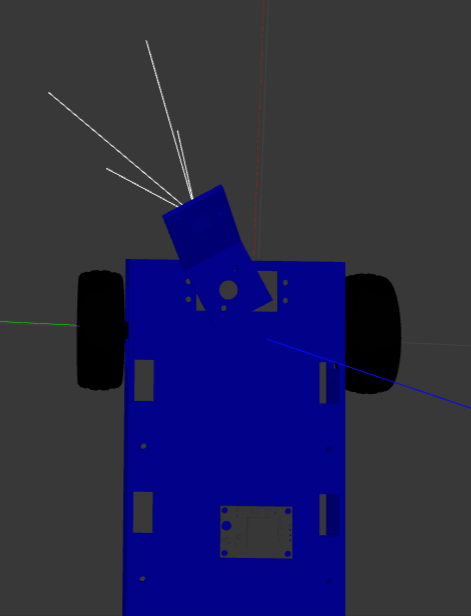
\includegraphics[width=\linewidth]{figs/cap6/rotizq.png}
		\caption*{\centering Rotación hacia la izquierda} 
	\end{minipage}
	\hspace{2cm}
	\begin{minipage}{0.35\linewidth}
		\centering
		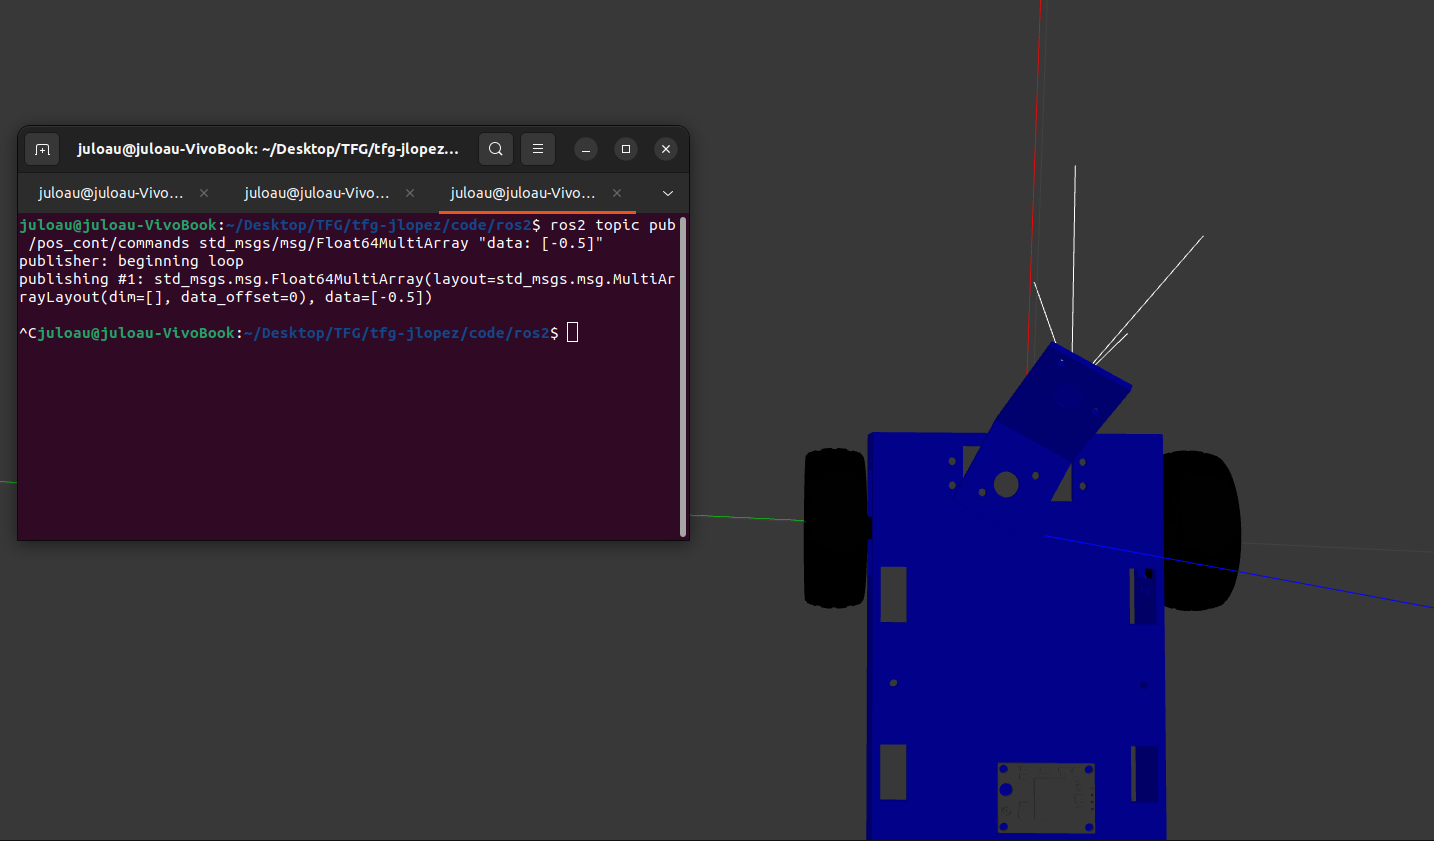
\includegraphics[width=\linewidth]{figs/cap6/rotder.png}
		\caption*{\centering Rotación hacia la derecha} 
	\end{minipage}
	\caption{Herramienta usada para rotar la cámara}
	\label{fig:camararot}
\end{figure}


%Una vez se ha demostrado el funcionamiento de PiBotJ en simulación con este video\footnote{\url{https://www.youtube.com/watch?v=A0yi7YlLpq0}}, ya se puede dar soporte al robot físico.

\section{Ejecución del robot real}
\label{sec:configrf}

Una vez definido el robot a través de sus topics, ya se puede lanzar su ejecución (usando la RPi 4 como núcleo computacional) para realizar su tarea.

%Como se explicó en la sección anterior, el robot ya estaba listo en simulación para, a través de los \textit{topics} definidos en el apartado anterior, poder definir y monitorear su comportamiento. Después de eso, era momento de poner al robot físico también listo para operar. 
El sistema operativo instalado en la placa controladora fue Ubuntu 20.04 Server \acs{LTS} y la distribución Foxy de ROS2, como se explicó en la Sección \ref{subsec:ubuntu} y \ref{subsec:ros2} respectivamente. Se hizo uso de SSH a efectos de usar el PC principal como cliente. Para ello, se instaló el paquete de openssh-client.

%En la Raspberry Pi se decidió instalar Ubuntu 20.04 Server \acs{LTS}, como se explicó en el Apartado \ref{subsec:ubuntu}, y para ello, fue necesario instalar en el ordenador principal, que actuaba como cliente, el siguiente programa:  \verb|sudo apt-get install openssh-client|. Como en Ubuntu 20.04 la distribución de ROS 2 era foxy, había que seguir los pasos de instalación de la Sección \ref{sec:simulacion} pero cambiando humble por foxy. 

%Por otro lado, ahora desde una terminal del ordenador, se puede conectar al robot a través de ssh, escribiendo \verb|ssh usuario@ip_dispositivo| y posteriormente, introduciendo la constraseña creada en el proceso de instalación. Esta era la forma de comunicación con el robot ya que esta distribución, no tenía interfaz gráfica. De las variante de ssh se usaba scp -r para copiar directorios entre el robot y el ordenador local y permitir subir los cambios a Github, y para desarrollar código se usaba un \textit{plugin} de VSCode que permite usar VSCode conectándose al robot usando ssh\footnote{\url{https://code.visualstudio.com/docs/remote/ssh-tutorial}}. 

Es importante recordar que, al usar ROS 2, todos los nodos que estén ejecutándose dentro de una red Wifi, serán visibles para cualquier dispositivo que esté conectado dentro de esa red Wifi. Gracias a eso, se facilitó la depuración y monitorización de cada sensor y actuador de PiBotJ. 

%En los siguientes apartados se detalla cómo se ha configurado cada dispositivo que conforma el PiBotJ.

En los siguientes apartados se detalla cómo cada dispositivo que conforma el PiBotJ está en funcionamiento. Para conocer todos los pasos seguidos para poder configurar cada componente, se puede ver en el \hyperref[cap:capitulo9]{Anexo}.  

%Una vez dentro del robot y conociendo todas las posibles formas de estar comunicados con él, era el momento de configurar cada dispositivo que conformaba a PiBotJ.

\subsection{Cámara}
\label{subsec:configcamara}

%La cámara está conectada al puerto CSI y, para hacerla funcionar, se necesitan los siguientes programas: 

%\begin{verbatim}
%	sudo apt-get install gstreamer1.0-tools \ 
%	gstreamer1.0-plugins-base gstreamer1.0-plugins-good \ 
%	gstreamer1.0-plugins-bad gstreamer1.0-plugins-ugly
%\end{verbatim}

%Una vez instalados, fue necesario editar el fichero \verb|/boot/firmware/config.txt| añadiendo \verb|start_x=1| al final y se tuvo que reiniciar la Raspberry Pi. Para comprobar que la configuración fue correcta, era necesario usar el comando \verb|v4l2-ctl --list-devices|  que comprueba la lista de dispositivos de video y media que están disponibles en el sistema. En la Figura \ref{fig:v4l2} se puede ver el resultado de dicho comando y  muestra que la cámara se encontraba conectada en el dispositivo \verb|/dev/video0|.

 
% \begin{figure} [h!]
%	\begin{center}
%		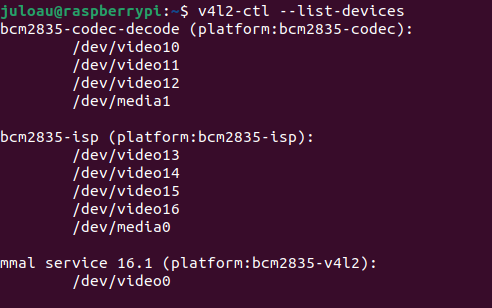
\includegraphics[width=9cm]{figs/cap6/vl.png}
%	\end{center}
%	\caption{Dispositivos de video y media disponibles en PiBotJ}
%	\label{fig:v4l2}
%\end{figure}


%Sabiendo que la cámara estaba disponible, era necesario comprobar que realmente la imagen se pudiera ver correctamente. Para ello, 

Partiendo del \verb|cameraPublisher.py| de este tutorial\footnote{\url{https://www.youtube.com/watch?v=6e94ZnYnO_U}}, se pudo crear un nodo llamado \verb|camera_node|\footnote{\url{https://github.com/RoboticsURJC/tfg-jlopez/blob/main/code/ros2/src/pibotj_rr/pibotj_rr/camera.py}} que permitía leer y publicar la imagen del dispositivo de la cámara. También se puede monitorizar usando las mismas herramientas que en la Sección \ref{subsec:funsimulacion} para controlar la cámara en simulación (Figura \ref{fig:camararr}).

 \begin{figure} [h!]
	\begin{center}
		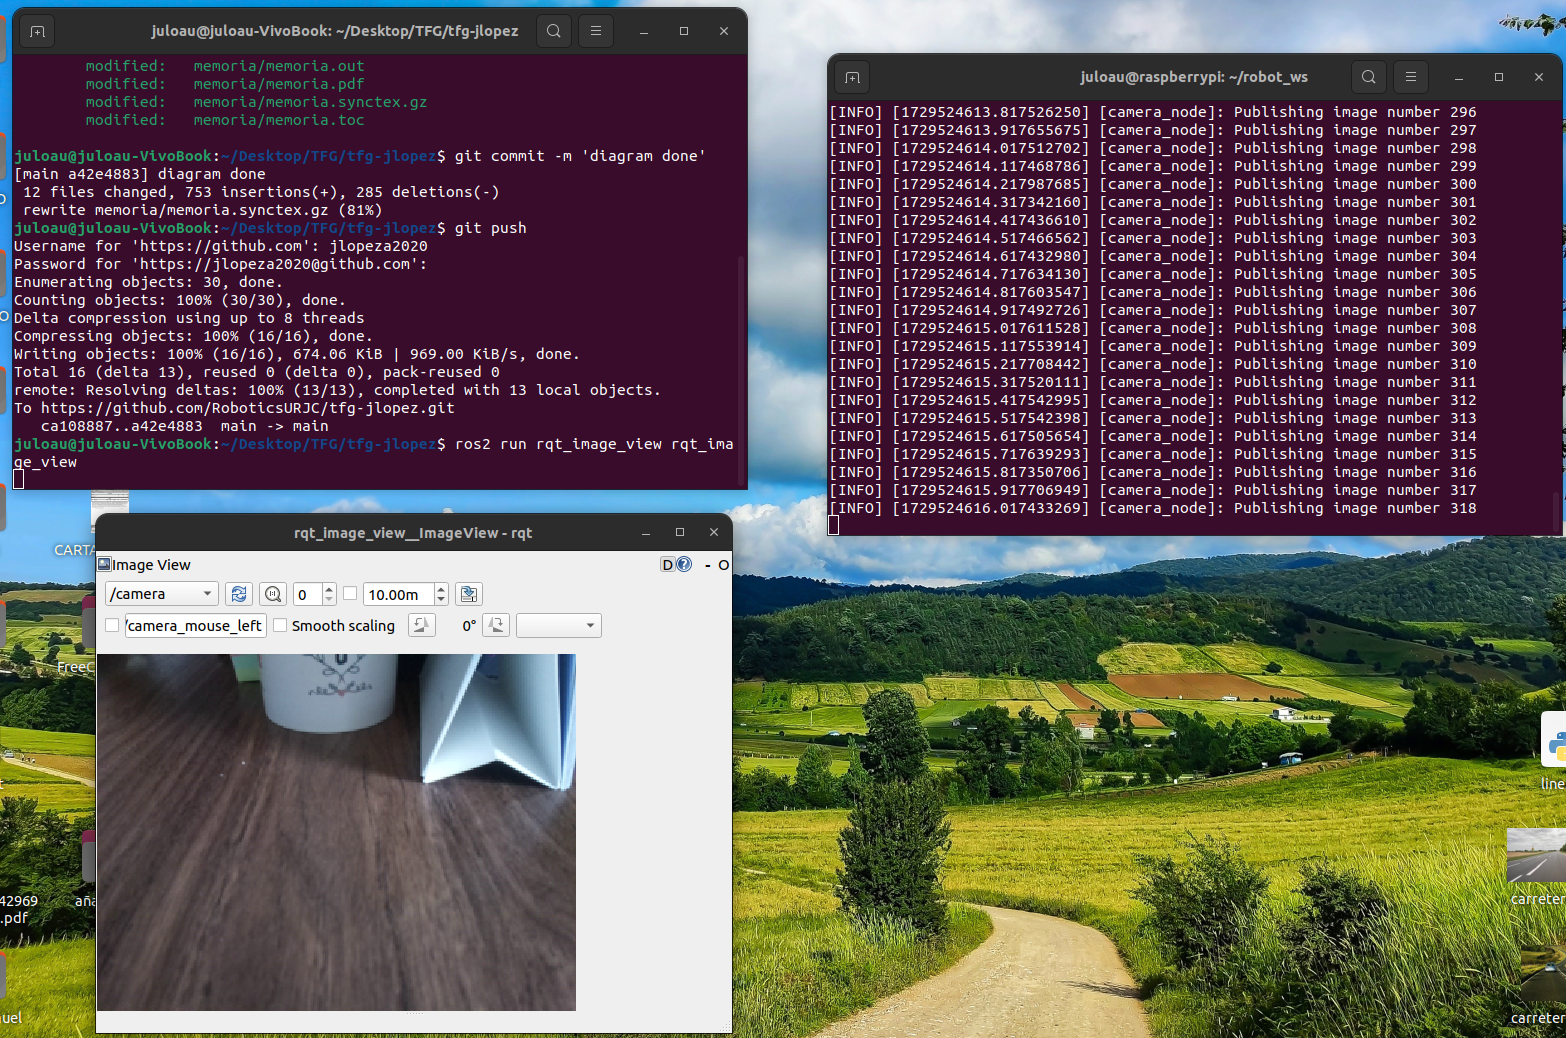
\includegraphics[width=8cm]{figs/cap6/camerarr.png}
	\end{center}
	\caption{Cámara de PiBotJ en funcionamiento}
	\label{fig:camararr}
\end{figure}

Para conformar un modelo teórico de la cámara se necesitan conocer sus parámetros intrínsecos y extrínsecos.
%Para posteriores cálculos, era necesario conocer tanto los parámetros intrínsecos como extrínsecos de la cámara.  

\subsubsection{Parámetros intrínsecos}
\label{subsubsec:intrinsecoscamara}

Los parámetros intrínsecos definen la geometría interna y la óptica de la cámara. Estos determinan cómo la cámara proyecta los puntos del mundo 3D al plano de la imagen en 2D, siendo constantes mientras no varíen las características y posiciones relativas entre la óptica y el sensor imagen. Estos parámetros los provee el fabricante de la cámara, aunque se pueden obtener mediante un proceso de calibración.

Para los cálculos teóricos se decidió consultar en numerosas fuentes de información y gracias a la Web \textit{Elinux}\footnote{\url{https://elinux.org/Rpi_Camera_Module\#Technical_Parameters_.28v.2_board.29}}, se pudieron obtener, sus parámetros técnicos. Asimismo, siguiendo el libro \cite{Hartley2004} se consiguieron las fórmulas correspondientes a la distancia focal (Ecuación \ref{ec:distfocal}) y al centro de la imagen (Ecuación \ref{ec:cenimagen}).


\begin{myequation}[h]
	\begin{align}
		f_x &= F \cdot \frac{\text{Res. horizontal}}{\text{tam. sensor horizontal}} \quad
		f_x = 3.04 \cdot \frac{640}{3.674} = 529,56 \\
		\hspace{1cm}
		f_y &= F \cdot \frac{\text{Res. vertical}}{\text{tam. sensor vertical}} \quad
		f_y = 3.04 \cdot \frac{480}{2.760} = 528,69
	\end{align}
	\caption[Fórmula para calcular la distancia focal teórica]{Fórmula para calcular la distancia focal teórica}
	\label{ec:distfocal}
\end{myequation}

\begin{myequation}[h]
	\begin{align}
		c_x &= \frac{\text{Res. horizontal}}{2} \quad
		c_x = \frac{640}{2} = 320 \\
		\hspace{1cm}
		c_y &= \frac{\text{Res. vertical}}{2} \quad
		c_y =  \frac{480}{2} = 240
	\end{align}
	\caption[Fórmula para calcular el centro de la imagen]{Fórmula para calcular el centro de la imagen}
	\label{ec:cenimagen}
\end{myequation}

Para los cálculos prácticos ha sido necesario seguir los pasos de calibración creando los ficheros \verb|calibration.py|\footnote{\url{https://github.com/RoboticsURJC/tfg-jlopez/blob/main/code/camera/calibration/calibration.py}} y \verb|process.py|\footnote{\url{https://github.com/RoboticsURJC/tfg-jlopez/blob/main/code/camera/calibration/process.py}} siguiendo el tutorial\footnote{\url{https://www.youtube.com/watch?v=XFBKwme5HYk}}. El fichero \verb|calibration.py| captura las imágenes con un patrón de ajedrez, y el fichero \verb|process.py| genera la matriz de parámetros intrínsecos y de distorsión. El proceso se repitió diez veces, siendo la matriz resultante la obtenida como media de las diez matrices. Sus valores son: $f_x$ = 497,66 , $f_y$ = 502,16 , $c_x$ = 325,3 y $c_y$ = 240,18 (Figura \ref{fig:meanintrinseco})

 \begin{figure} [h!]
	\begin{center}
		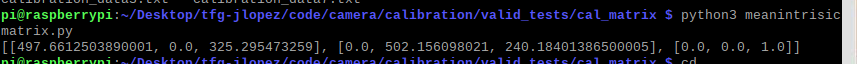
\includegraphics[width=15cm]{figs/cap6/intrinsicmedia.png}
	\end{center}
	\caption{Media de la matriz de intrínsecos}
	\label{fig:meanintrinseco}
\end{figure}


Podemos ver que los valores de fábrica difieren de los obtenidos empíricamente. Esto es debido a que cada cámara tiene sus pequeñas diferencias, propias del proceso de calibración.


\subsubsection{Parámetros extrínsecos}
\label{subsubsec:extrinsecoscamara}

Los parámetros extrínsecos relacionan los sistemas de referencia del mundo real y la cámara, describiendo la posición y orientación de la cámara en el sistema de coordenadas del mundo real. Dichos parámetros incluyen la rotación y la traslación de la cámara. En este caso, la cámara tiene una rotación sobre el eje Y de 50º (Figura \ref{fig:extrinseco} izquierda) y está trasladada 8,8 cm en el eje Z (Figura \ref{fig:extrinseco} derecha). 

\begin{figure}[ht!]
	\centering
	\begin{minipage}{0.35\linewidth}
		\centering
		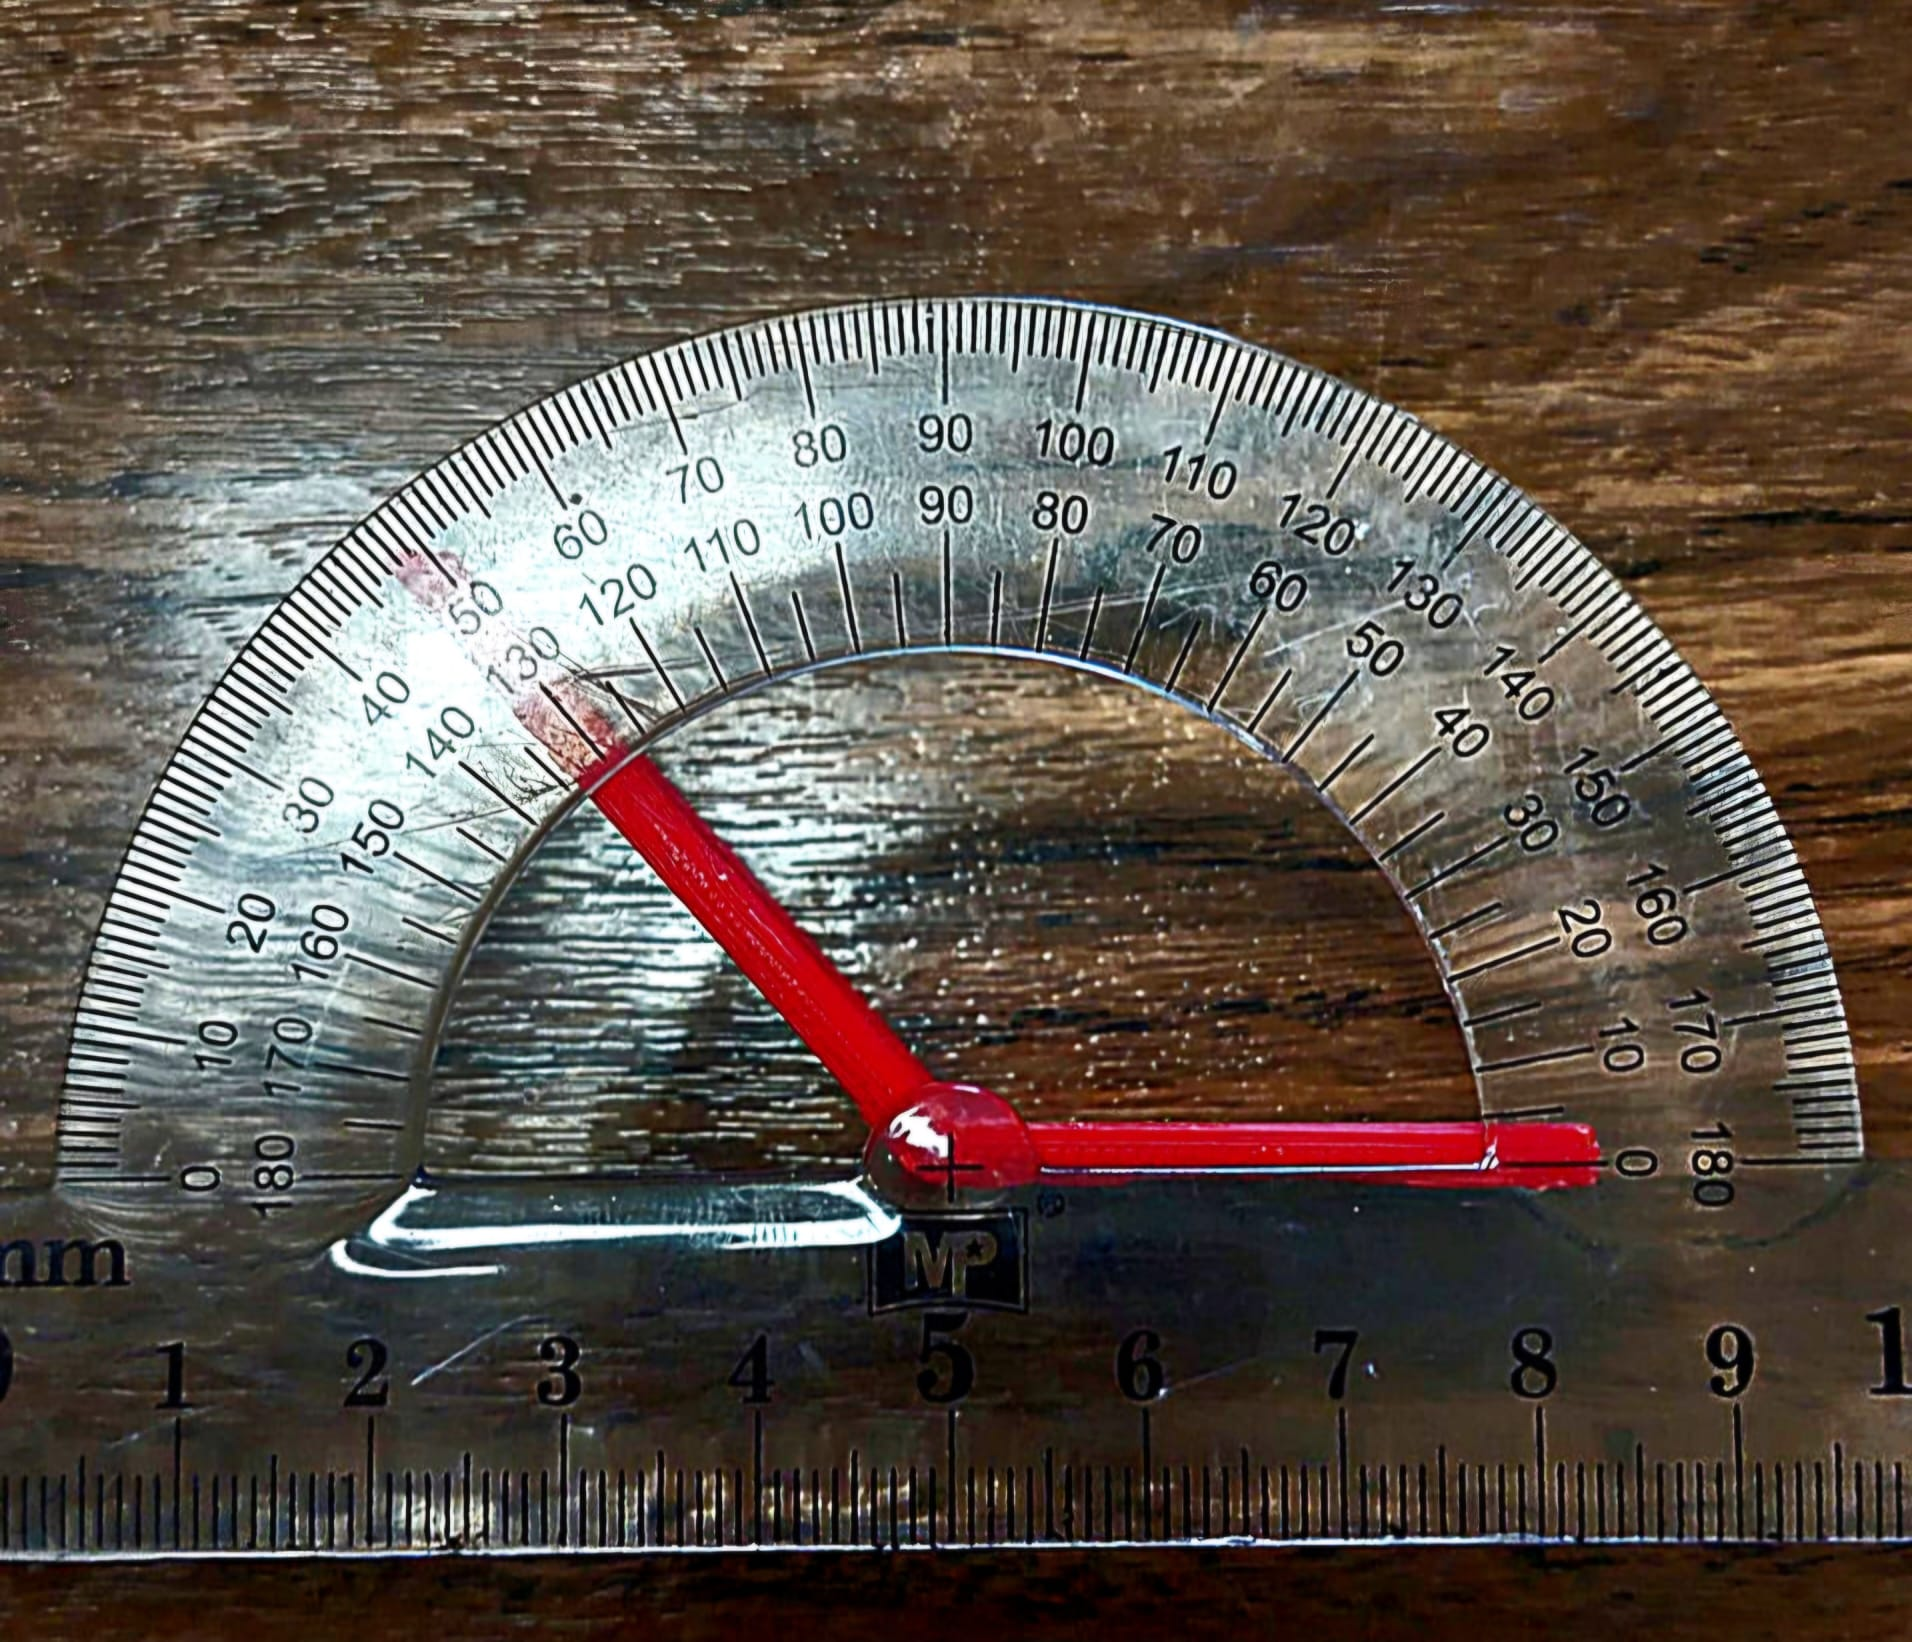
\includegraphics[width=\linewidth]{figs/cap6/rotation.jpeg}
		\caption*{\centering Rotación de la cámara} 
	\end{minipage}
	\hspace{2 cm}
	\begin{minipage}{0.35\linewidth}
		\centering
		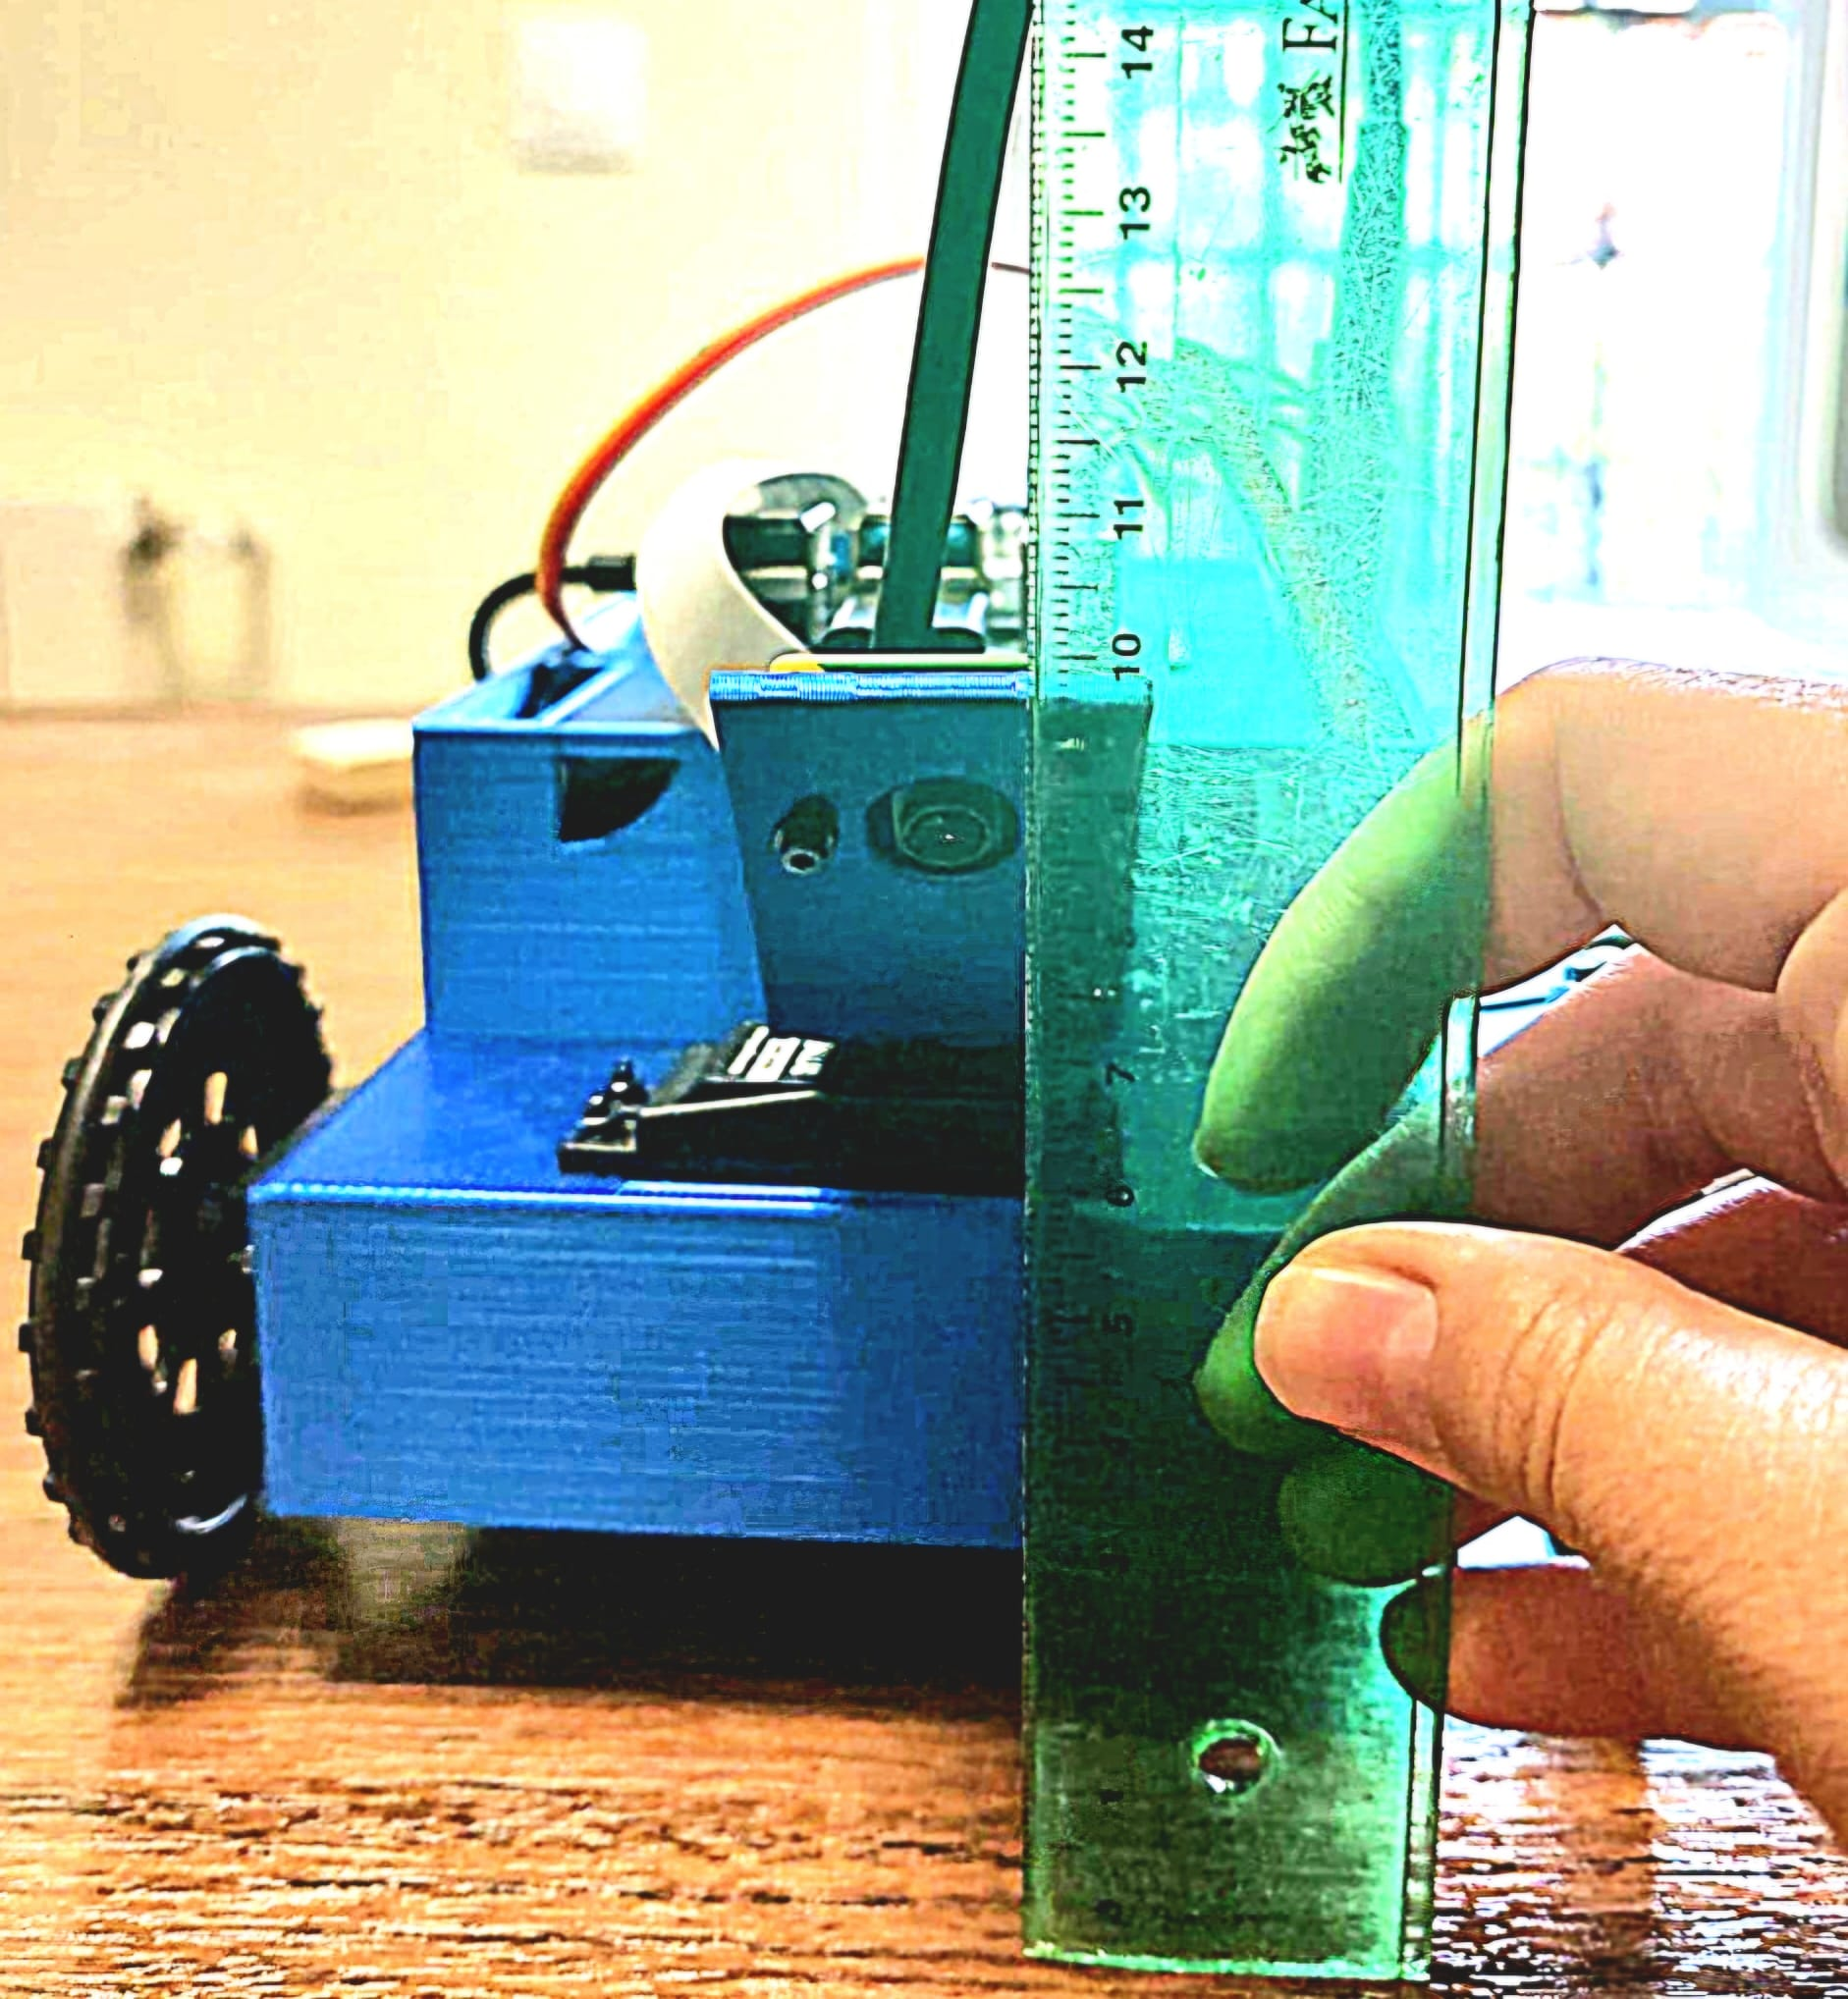
\includegraphics[width=\linewidth]{figs/cap6/traslacion.jpeg}
		\caption*{\centering Traslación de la cámara} 
	\end{minipage}
	\caption{Parámetros extrínsecos}
	\label{fig:extrinseco}
\end{figure}


\subsection{Google Coral USB}
\label{subsec:configgcoral}

Como se comentó en la Sección \ref{subsec:googlecoral}, existen severas limitaciones al tratar de acelerar tareas en dispositivos que no cuentan con hardware específico para ello. Por ello, se decidió incluir el dispositivo USB Google Coral y se puede demostrar que está en funcionamiento si la luz que tiene el dispositivo parpadea. 

%Para su configuración se han seguido los pasos indicados en su web oficial\footnote{\url{https://coral.ai/docs/accelerator/get-started/}}. 

%Una vez la cámara estaba lista para operar y se conoce que existen muchas limitaciones cuando se trata de acelerar tareas en dispositivos que no cuentan con \textit{hardware} para ello, como se comentó en el Apartado \ref{subsec:googlecoral}, se decidió incluir el dispositivo USB Google Coral y para ello, es necesario configurarlo.

%En su web oficial\footnote{\url{https://coral.ai/docs/accelerator/get-started/}} se pueden encontrar diferentes pasos de instalación dependiendo de las necesidades del usuario, pero se pueden resumir para cumplir con las características de la arquitectura de este dispositivo de la siguiente manera:

%
%\begin{lstlisting}[language=bash]
%	echo "deb https://packages.cloud.google.com/apt \
%	coral-edgetpu-stable main" | \
%	sudo tee /etc/apt/sources.list.d/coral-edgetpu.list
	
%	curl https://packages.cloud.google.com/apt/doc/apt-key.gpg \
%	| sudo apt-key add -
	
%	sudo apt-get update	
%	sudo apt-get install libedgetpu1-std
	
%	# Conecta el USB en uno de los puertos 3.0
	
%	sudo apt-get install python3-pycoral
%\end{lstlisting}

%Finalmente, el proceso se debería haber completado cuando la salida del último comando se debería ver como muestra la Figura \ref{fig:outcoral}.

 %\begin{figure} [h!]
%	\begin{center}
%		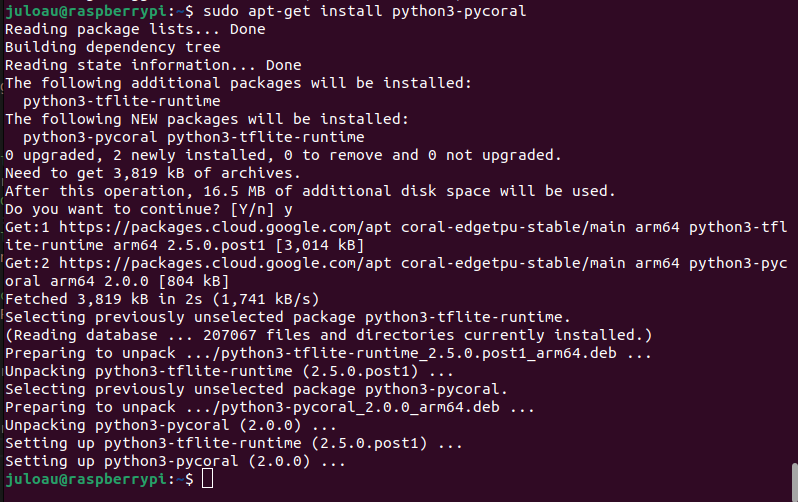
\includegraphics[width=12cm]{figs/cap6/pycoralinstalled.png}
%	\end{center}
%	\caption{Configuración exitosa del Google Coral}
%	\label{fig:outcoral}
%\end{figure}


\subsection{Módulo GPS}
\label{subsec:configgps}

El módulo \acs{GPS} utiliza una comunicación \acs{UART}, o comunicación serial, mediante puerto de transmisión TX y puerto de recepción RX. En nuestro caso, se utilizan los pines tratados en la Sección \ref{sec:disposicionhardware}.


%La estructura seguida en este tutorial\footnote{\url{https://sparklers-the-makers.github.io/blog/robotics/use-neo-6m-module-with-raspberry-pi/}} ha sido de gran ayuda para configurar el módulo \acs{GPS} que, para esta arquitectura, supone seguir los siguientes pasos: 

%Crea el fichero \verb|/etc/udev/rules.d/99-ttyAMA0.rules| que tiene que contener: \verb|KERNEL=="ttyAMA0", MODE="0666", GROUP="dialout"| y para que se actualicen en el sistema es necesario recargar las reglas, escribiendo por terminal lo siguiente: 

%\begin{verbatim}
%	sudo udevadm control --reload-rules
%	sudo udevadm trigger
%\end{verbatim}

%Como esta distribución no tiene interfaz web, no tiene instalado por defecto \verb|raspi-config|. Así, para su instalación se ha seguido el siguiente tutorial\footnote{\url{https://github.com/EmilGus/install_raspi-config/tree/master}} y, una vez instalado, hay que ejecutarlo usando \verb|sudo raspi-config|. Dentro de \textit{raspi-config} hay que desplazarse hasta \textit{Interfacing options} y \textit{serial}, hay que desabilitar \textit{serial login shell}, habilitar \textit{serial interface} y reiniciar con \verb|sudo reboot|.

%Finalmente los siguientes ficheros tienen que contener la siguiente información: 


%\begin{lstlisting}[language=bash]
%cat /boot/firmware/config.txt 

%# Please DO NOT modify this file; if you need to modify the boot config,
%# the "usercfg.txt" file is the place to include user changes. Please 
%# refer to the README file for a description of the various configuration 
%# files on the boot partition.

%# The unusual ordering below is deliberate; older firmwares (in particular 
%# the version initially shipped with bionic) don't understand the conditional
%# [sections] below and simply ignore them. The Pi4 doesn't boot at all 
%# with firmwares this old so it's safe to place at the top. Of the Pi2 and 
%# Pi3, the Pi3 uboot happens to work happily on the Pi2, so it needs to go 
%# at the bottom to support old firmwares.

%[pi4]
%kernel=uboot_rpi_4.bin

%[pi2]
%kernel=uboot_rpi_2.bin

%[pi3]
%kernel=uboot_rpi_3.bin

%[pi0]
%kernel=uboot_rpi_3.bin

%[all]
%device_tree_address=0x03000000

%[pi4]
%max_framebuffers=2
%arm_boost=1

%[all]
%# Enable the audio output, I2C and SPI interfaces on the GPIO header. As these
%# parameters related to the base device-tree they must appear *before* any
%# other dtoverlay= specification
%dtparam=audio=on
%dtparam=i2c_arm=on
%dtparam=spi=on

%# Comment out the following line if the edges of the desktop appear outside
%# the edges of your display
%disable_overscan=1

%# If you have issues with audio, you may try uncommenting the following line
%# which forces the HDMI output into HDMI mode instead of DVI (which doesn't
%# support audio output)
%#hdmi_drive=2

%# Config settings specific to arm64
%arm_64bit=1
%dtoverlay=dwc2

%[cm4]
%# Enable the USB2 outputs on the IO board (assuming your CM4 is plugged into
%# such a board)
%dtoverlay=dwc2,dr_mode=host

%[all]

%# The following settings are "defaults" expected to be overridden by the
%# included configuration. The only reason they are included is, again, to
%# support old firmwares which don't understand the "include" command.

%enable_uart=1
%cmdline=cmdline.txt

%include syscfg.txt
%include usercfg.txt

%start_x=1
%\end{lstlisting}

%\begin{lstlisting}[language=bash]
%cat /boot/firmware/cmdline.txt 

%elevator=deadline net.ifnames=0 dwc_otg.lpm_enable=0 root=LABEL=writable \
% rootfstype=ext4 rootwait fixrtc quiet splash cfg80211.ieee80211_regdom=GB
%\end{lstlisting}

%\begin{lstlisting}[language=bash]
%cat /boot/firmware/usercfg.txt 
	
%# Place "config.txt" changes (dtparam, dtoverlay, disable_overscan, etc.) in
%# this file. Please refer to the README file for a description of the various
%# configuration files on the boot partition.
%dtoverlay=pi3-disable-bt
%\end{lstlisting}

%\begin{lstlisting}[language=bash]
% cat /boot/firmware/syscfg.txt 
 
%# This file is intended to be modified by the pibootctl utility. User
%# configuration changes should be placed in "usercfg.txt". Please refer to the
%# README file for a description of the various configuration files on the boot
%# partition.

%enable_uart=1
%dtparam=audio=on
%dtparam=i2c_arm=on
%dtparam=spi=on
%cmdline=cmdline.txt	
%\end{lstlisting}


El serial se encuentra configurado correctamente en \verb|/dev/ttyAMA0| gracias a los pasos de instalación descritos en el \hyperref[cap:capitulo9]{Anexo}, como muestra la Figura \ref{fig:nmea}. Para tratar la información obtenida, se decidió usar la librería llamada PyNMEA2, detallada en la Sección \ref{subsec:pynmea}, y que se desarrolló con el código del nodo \verb|gps_node|\footnote{\url{https://github.com/RoboticsURJC/tfg-jlopez/blob/main/code/ros2/src/pibotj_rr/pibotj_rr/gps_node.py}} para parsear la información y únicamente publicar la latitud y longitud, como muestra la Figura \ref{fig:gpsnode}. De los valores obtenidos, se decidió usar un conversor de coordenadas\footnote{\url{https://www.coordenadas-gps.com/convertidor-de-coordenadas-gps}} para demostrar que los valores recibidos eran correctos, como muestra la Figura \ref{fig:demogpsnode}.


 \begin{figure} [h!]
	\begin{center}
		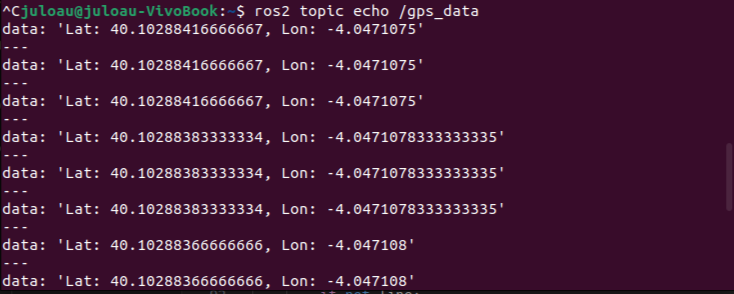
\includegraphics[width=12cm]{figs/cap6/echo_gps_controller.png}
	\end{center}
	\caption{Valores publicados de latitud y longitud captados del GPS}
	\label{fig:gpsnode}
\end{figure}


 \begin{figure} [h!]
	\begin{center}
		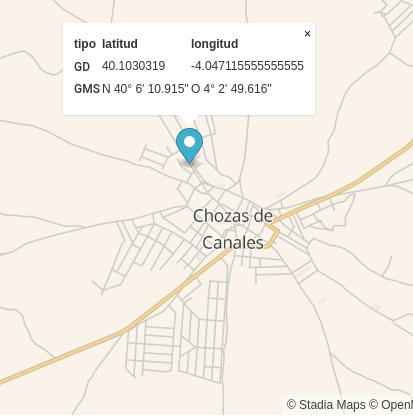
\includegraphics[width=15cm]{figs/cap6/localizacion.png}
	\end{center}
	\caption{Demostración de una correcta localización}
	\label{fig:demogpsnode}
\end{figure}

%% Preguntar si dejarlo o no
Debido a la distribución de Ubuntu usada, hay problemas al encender la Raspberry Pi si tiene algo a través del puerto serie\footnote{\url{https://wiki.ubuntu.com/EoanErmine/ReleaseNotes\#Raspberry_Pi}}, pero las sugerencias de otros usuarios no conseguían hacer funcionar bien el módulo; por lo tanto, la única solución encontrada fue desconectar el módulo \acs{GPS} hasta que se inicia sesión a través de ssh y luego conectar el módulo.

El módulo GPS realmente capta información válida cuando se enciende el LED azul que tiene integrado. Una forma fiable para que el módulo reciba todo el rato señal correcta es dejarle en el exterior hasta que se encienda el LED y luego poder operar con el módulo en interior o exterior. 


\subsection{Servomotores}
\label{subsec:configmotores}

Los últimos componentes que faltaban por configurar son los motores, que van conectados a los pines GPIO 
%y para ello hay que instalar los siguientes programas\footnote{\url{https://cms.gutow.uwosh.edu/Gutow/useful-chemistry-links/software-tools-and-coding/computer-and-coding-how-tos/allowing-access-to-gpio-i2c-and-spi-on-pi-under-ubuntu-20.04}}: 

%\begin{verbatim}
%	sudo apt-get update
%	sudo apt-get install rpi.gpio-common python3-pigpio python3-gpiozero \
%	 python3-rpi.gpio
%\end{verbatim}

%Para asegurarnos que funcionaban perfectamente habia que añadir \textit{dialout} a \textit{groups} y ya 
Tras seguir los pasos de configuración del \hyperref[cap:capitulo9]{Anexo}, importando la librería \verb|RPi.GPIO| se pueden operar directamente. Estos servomotores se mueven por posición entre 0º y 180º, y se controlan mediante modulación del ancho del pulso (\ac{PWM}), donde la posición del eje del servo depende de la duración del pulso. Para mantener su posición, el servo necesita recibir un pulso cada 20 ms\footnote{\url{https://docs.rs-online.com/0e85/0900766b8123f8d7.pdf}} (Figura \ref{fig:pwm}). Para cambiar ese \ac{PWM}\footnote{\url{https://solectroshop.com/es/blog/que-es-pwm-y-como-usarlo--n38}} es necesario usar el procedimiento \verb|ChangeDutyCycle()|, que modifica el porcentaje de tiempo que la señal está activa durante un período de la señal. En este caso, el ciclo de trabajo determina la posición del eje del servo siendo 0º de 2,5\% de \textit{duty cycle} y 180º de 12,5\% \textit{duty cycle}. Para facilitar la lógica de movimiento se creó una fórmula de conversión de grados a porcentaje de trabajo. En la Figura \ref{fig:motorlogic} se muestran los distintos valores necesarios para hacer los movimientos que necesitaba PiBotJ: hacia adelante, hacia atrás, girar hacia la izquierda mientras avanza hacia adelante, y girar hacia la derecha mientras avanza hacia adelante.

 \begin{figure} [h!]
	\begin{center}
		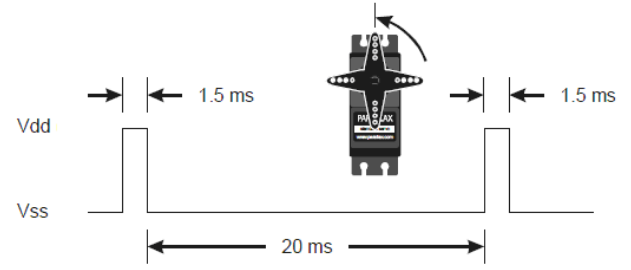
\includegraphics[width=12cm]{figs/cap6/pwm.png}
	\end{center}
	\caption{Diagrama para la posición central del servo}
	\label{fig:pwm}
\end{figure}

 \begin{figure} [h!]
	\begin{center}
		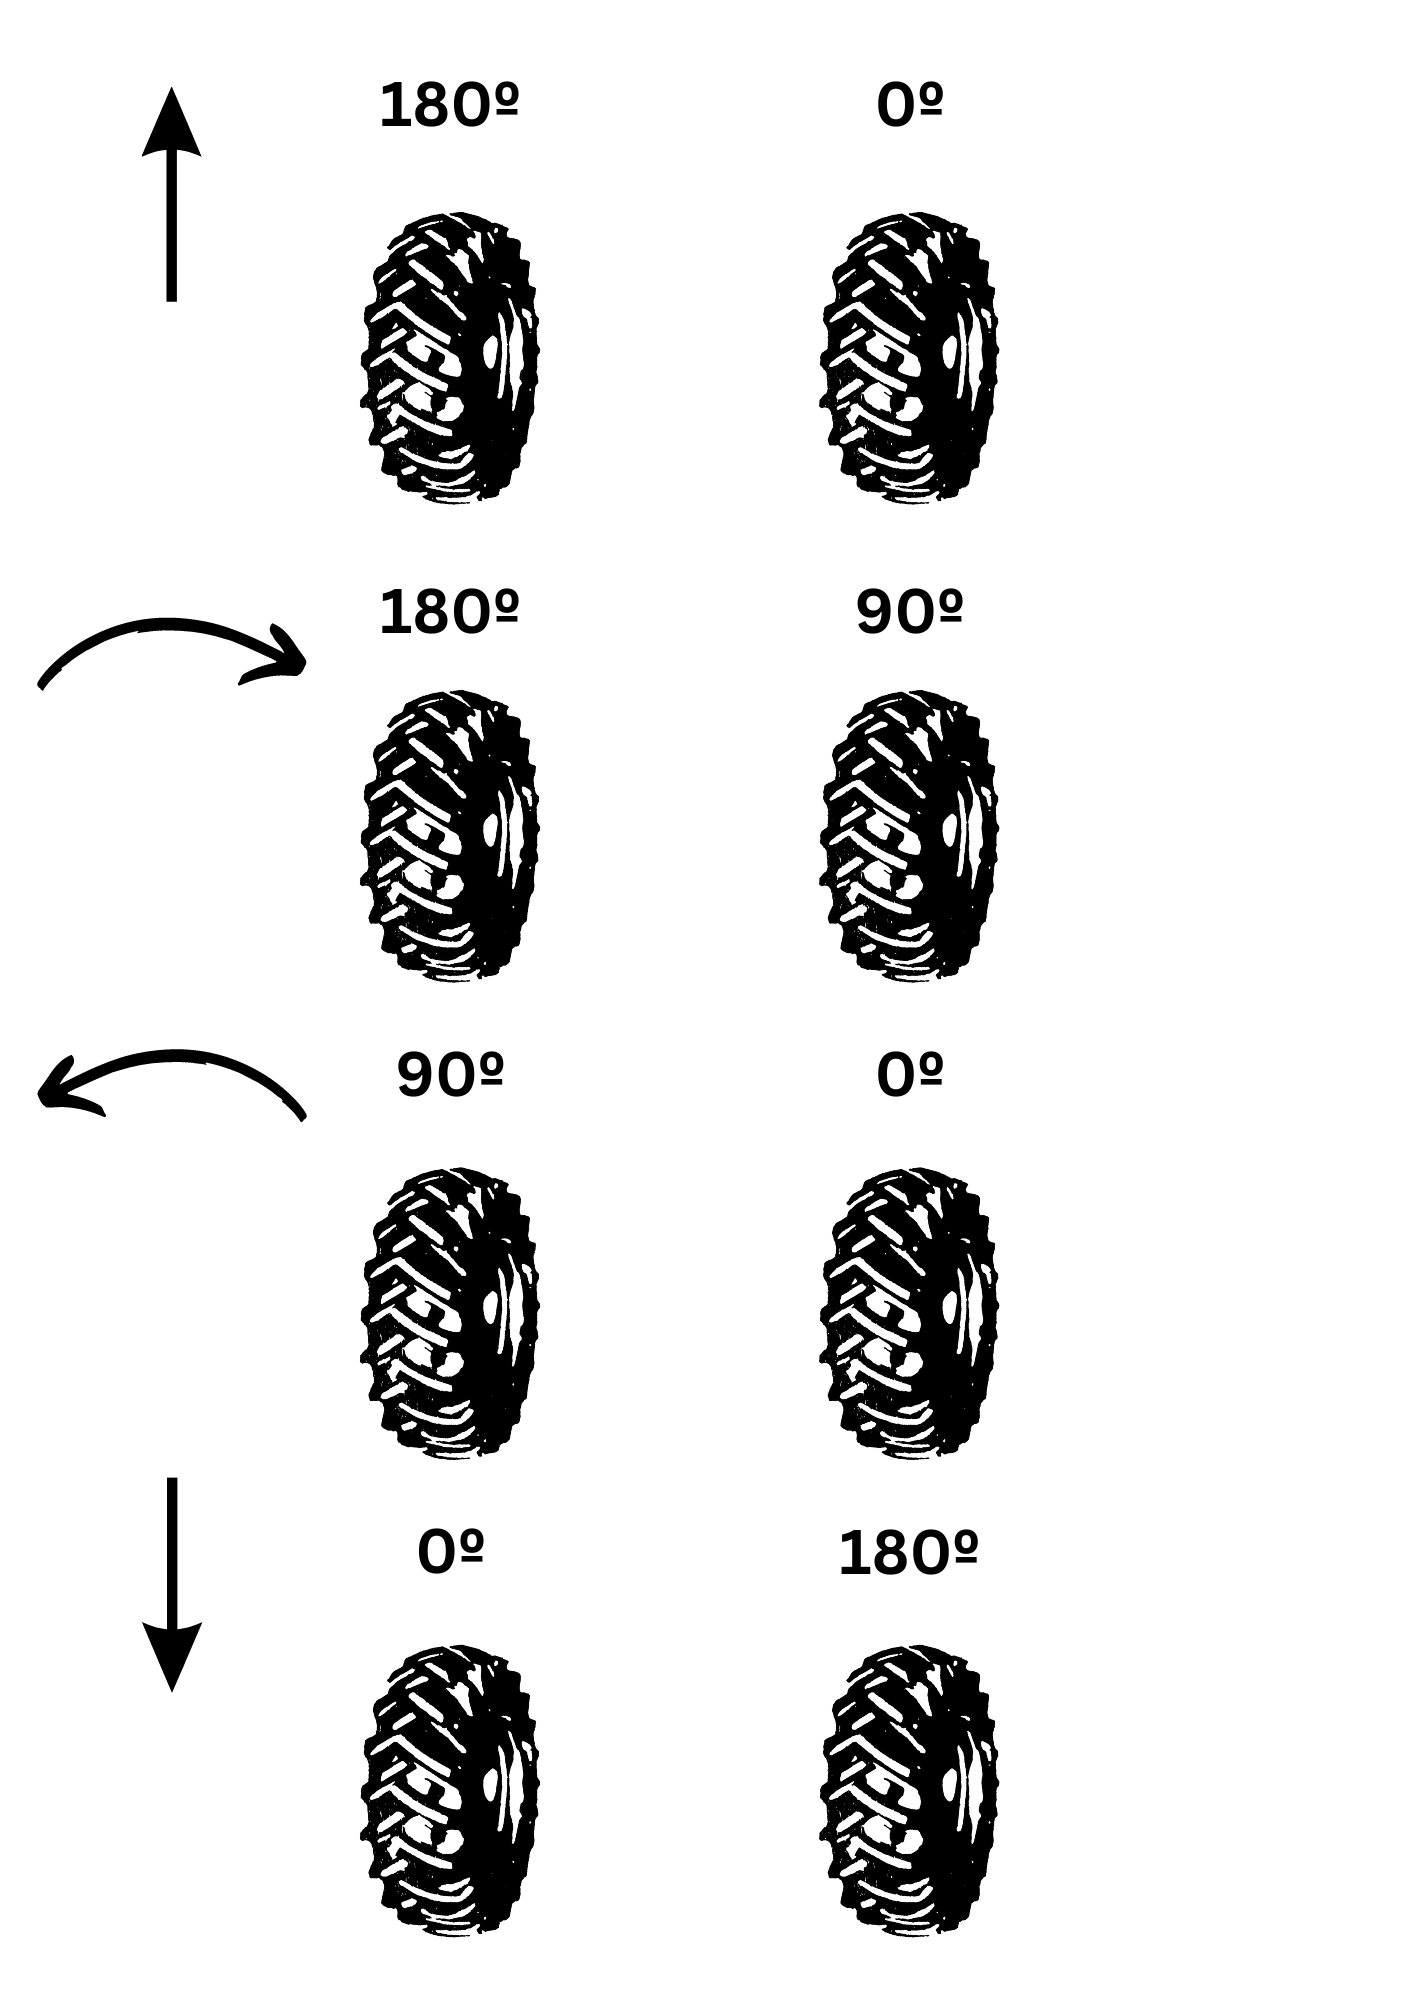
\includegraphics[width=6cm]{figs/cap6/motorlogic.png}
	\end{center}
	\caption{Distintas direcciones de PiBotJ}
	\label{fig:motorlogic}
\end{figure}\

Una vez configurados todos los componentes del robot, ya se puede pasar a desarrollar el \textit{software} que conforma el comportamiento final de este. 
 

\section{Software aplicado al robot físico}
\label{sec:softwarerf}

PiBotJ ya estaba listo para poder recibir la inteligencia que necesitaba para conseguir el objetivo principal descrito en la Sección \ref{sec:descripcion}. A diferencia de la Sección \ref{subsec:cap6ros2control} que empleaba ROS 2 control, en este caso al estar todo configurado a bajo nivel, se decidió usar una arquitectura de nodos con \textit{topics} publicadores y suscriptores.

\subsection{Red neuronal para la detección de baches}
\label{subsec:softwareiayolo}

Para conseguir la detección, se procedió al entrenamiento de un modelo de aprendizaje supervisado que detectaba baches. Se decidió usar YOLOv8, el cual hace uso de una única red neuronal convolucional para detectar objetos en imágenes en tiempo real y con facilidad de exportación a diferentes dispositivos.

Para poder entrenar dicho modelo, fue necesario usar un \textit{dataset} tomado de \cite{pothole-detection-project-new_dataset} que estaba formado por 202 imágenes ya segmentadas. El entrenamiento duró alrededor de una hora y con una duración de 120 \textit{epochs}. Una vez pasada esa hora, se pudo obtener el modelo entrenado en formato .pt y todos los resultados del entrenamiento aparecen mostrados en la Figura \ref{fig:iares} y \ref{fig:iares2}.

 \begin{figure} [h!]
	\begin{center}
		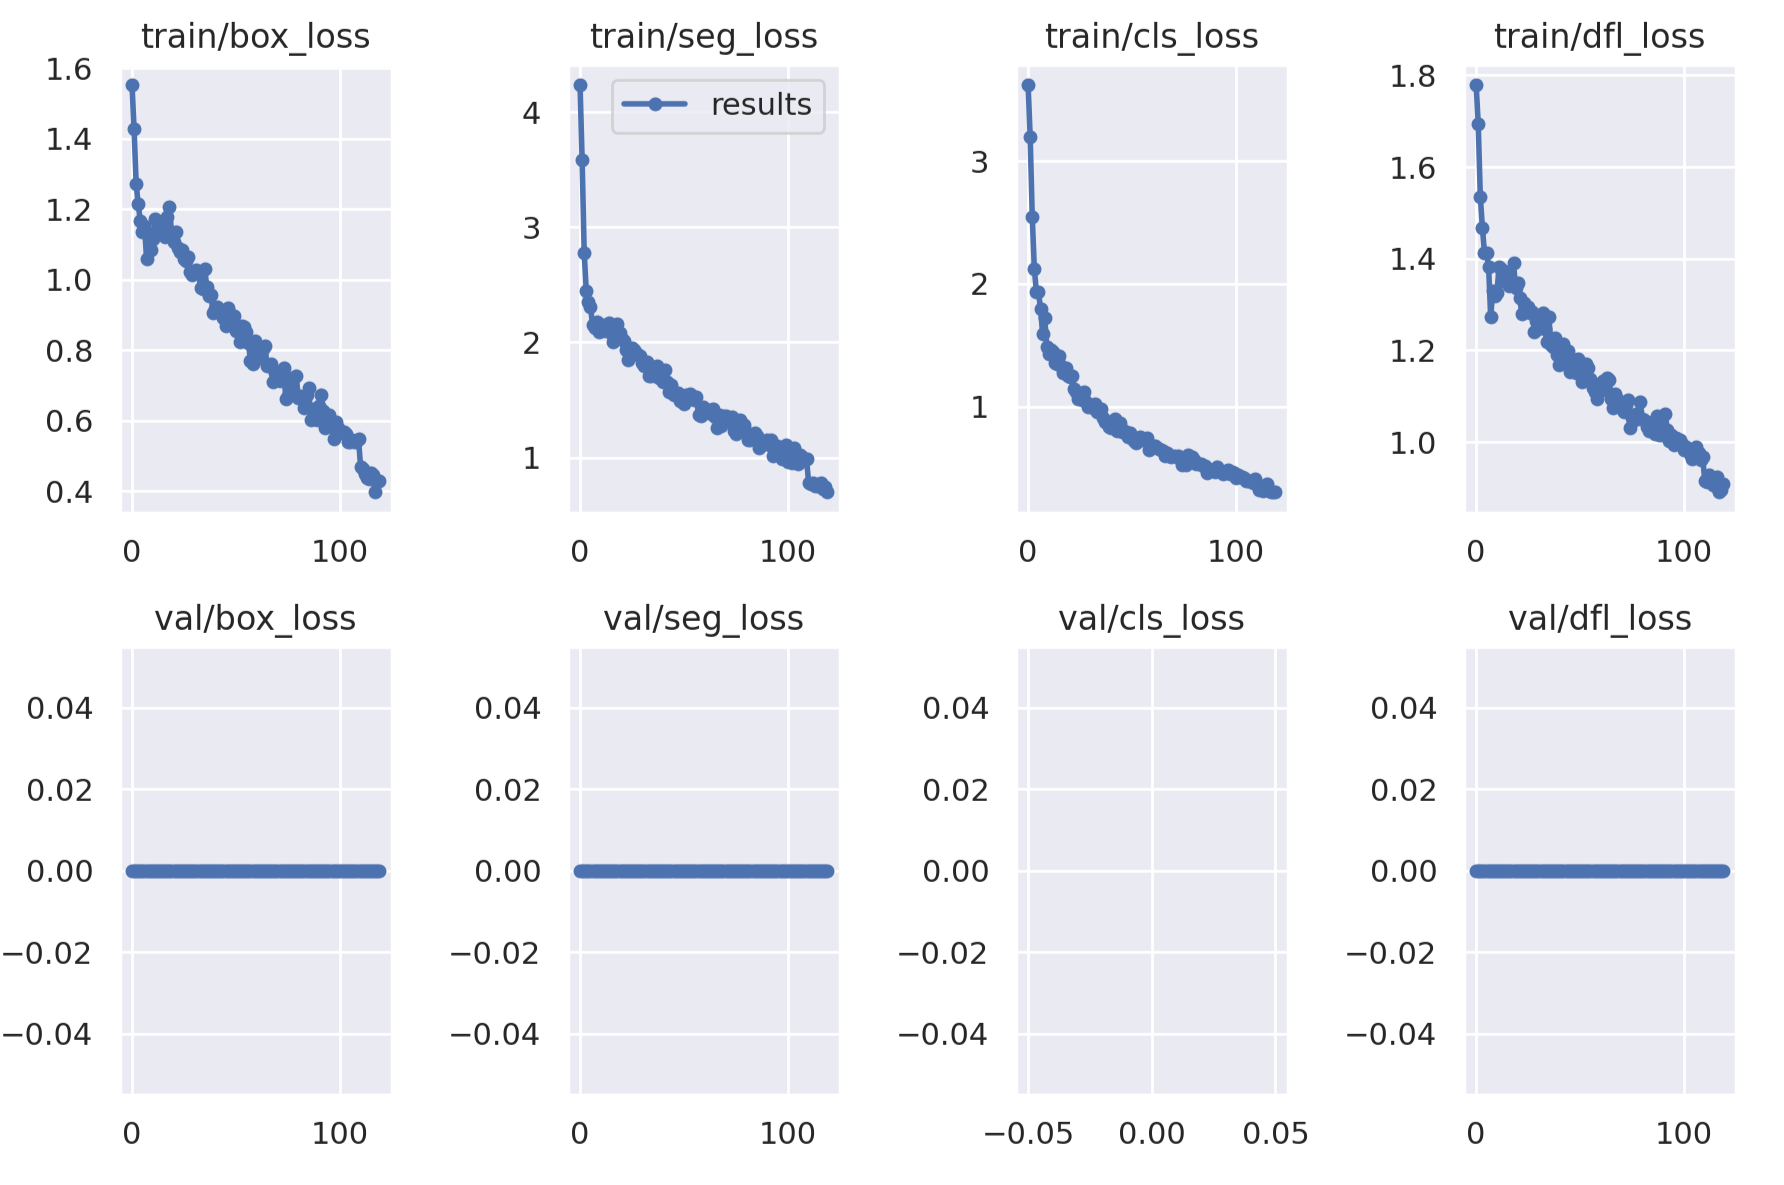
\includegraphics[width=15cm]{figs/cap6/results.png}
	\end{center}
	\caption{Gráficas de resultados del entrenamiento}
	\label{fig:iares}
\end{figure}


 \begin{figure} [h!]
	\begin{center}
		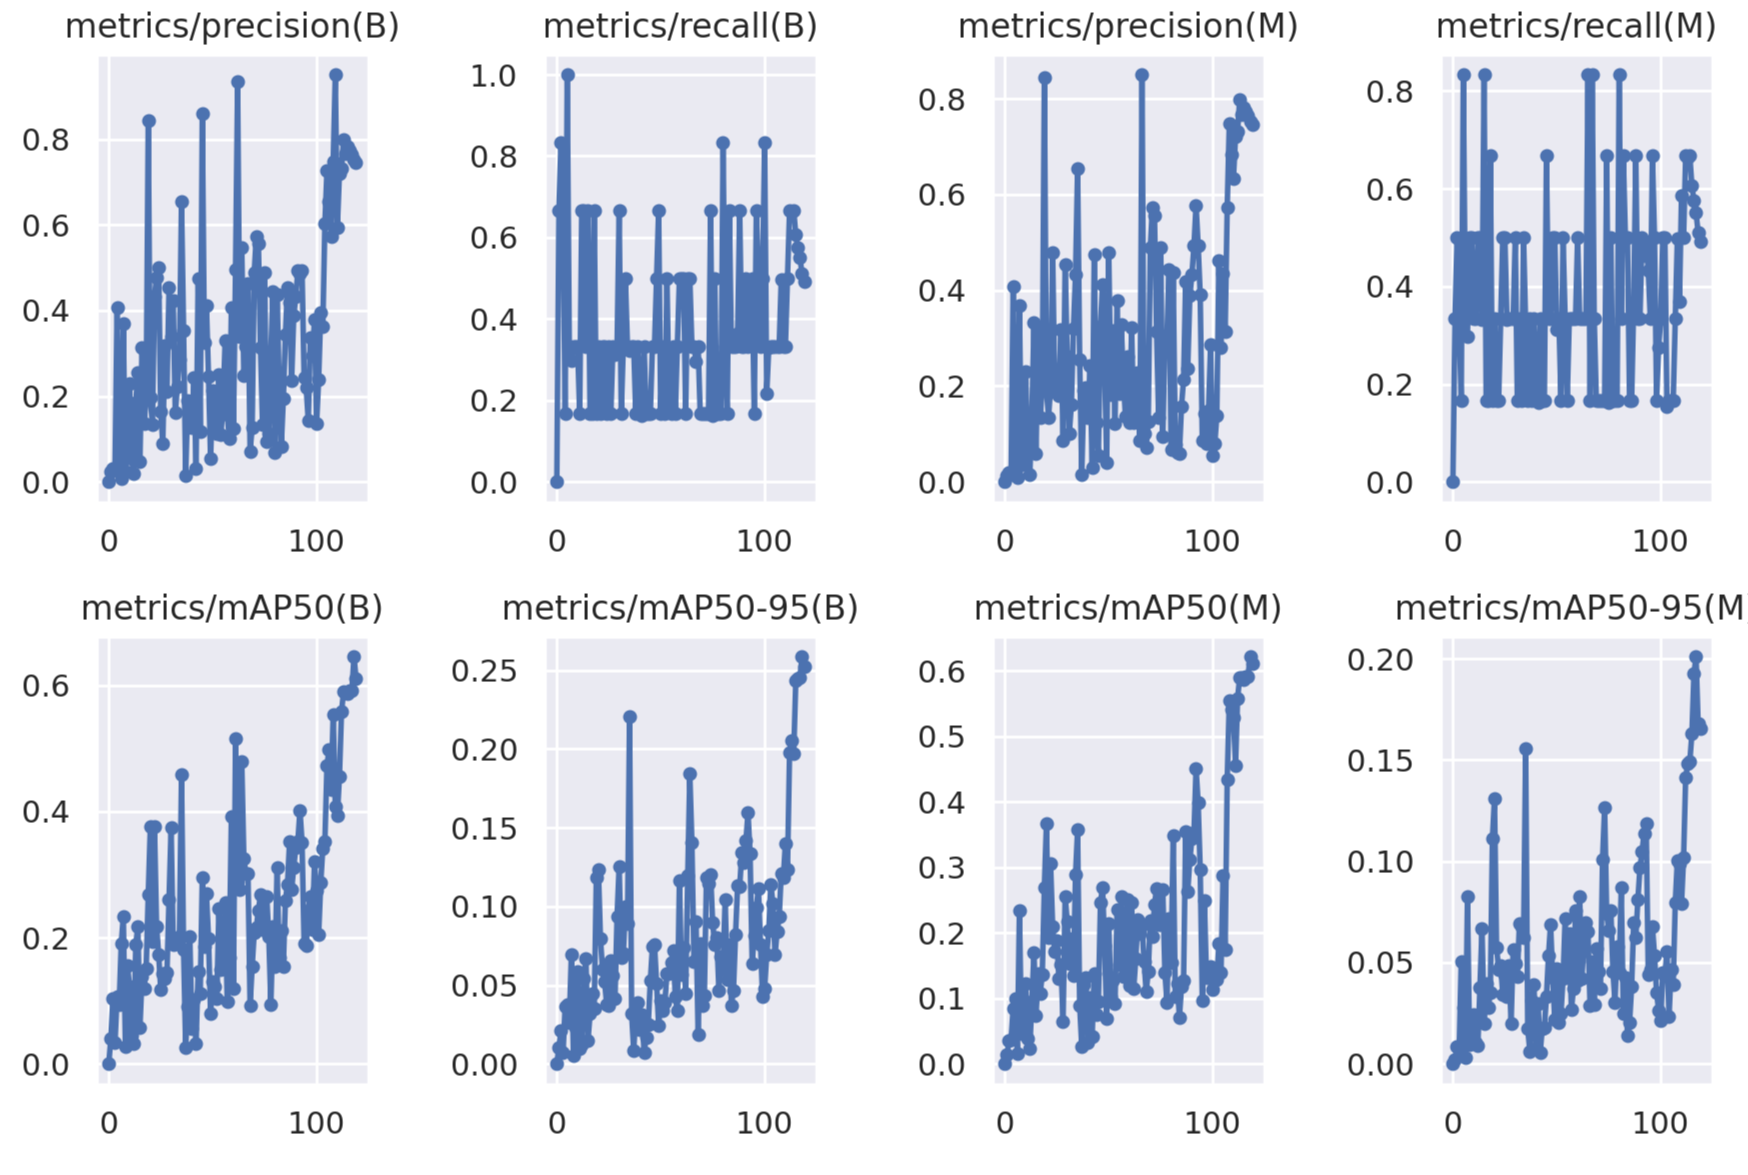
\includegraphics[width=15cm]{figs/cap6/results1.png}
	\end{center}
	\caption{Gráficas de resultados del entrenamiento: métricas}
	\label{fig:iares2}
\end{figure}

En la Figura \ref{fig:iares} se puede ver que aparecen cuatro gráficas en la parte superior midiendo el error obtenido durante el entrenamiento del modelo y se puede apreciar que disminuye a medida que pasa el tiempo y por lo tanto, se puede decir que existe un correcto entrenamiento. Por otro lado, las cuatro imágenes que aparecen debajo se tratan de las pérdidas calculadas en el conjunto de validación. Si las pérdidas en validación aumentan mientras las pérdidas de entrenamiento disminuyen, puede ser una señal de \textit{overfitting} (sobreajuste), en este caso al solo usar una imagen de validación el valor permanece constante sobre el 0.

En la Figura \ref{fig:iares2}, en concreto en la parte superior, se puede ver las métricas de precisión y exhaustividad (\textit{recall}) que evalúan la capacidad del modelo para identificar correctamente las instancias de cada clase ya que valores son crecientes. En la parte inferior, la métrica \ac{mAP} es creciente e indica que el modelo está mejorando en la detección y clasificación ya que, evalúa el equilibrio entre precisión y exhaustividad.

Para comprobar que el modelo funciona correctamente, se ha aplicado sobre una serie de imágenes mostradas en la Figura \ref{fig:trainex} y sobre un video\footnote{\url{https://www.youtube.com/watch?v=Gnwciv4pWf0}}. Todo está documentado en un Jupyter notebook\footnote{\url{https://colab.research.google.com/drive/1QRFWn5tQNXs6ldnomCZNv3DUDi8FudW2?usp=sharing}} basado en el tutorial de Muhammad Moin\footnote{\url{https://www.youtube.com/watch?v=bAlObHUIErM}}.

 \begin{figure} [h!]
	\begin{center}
		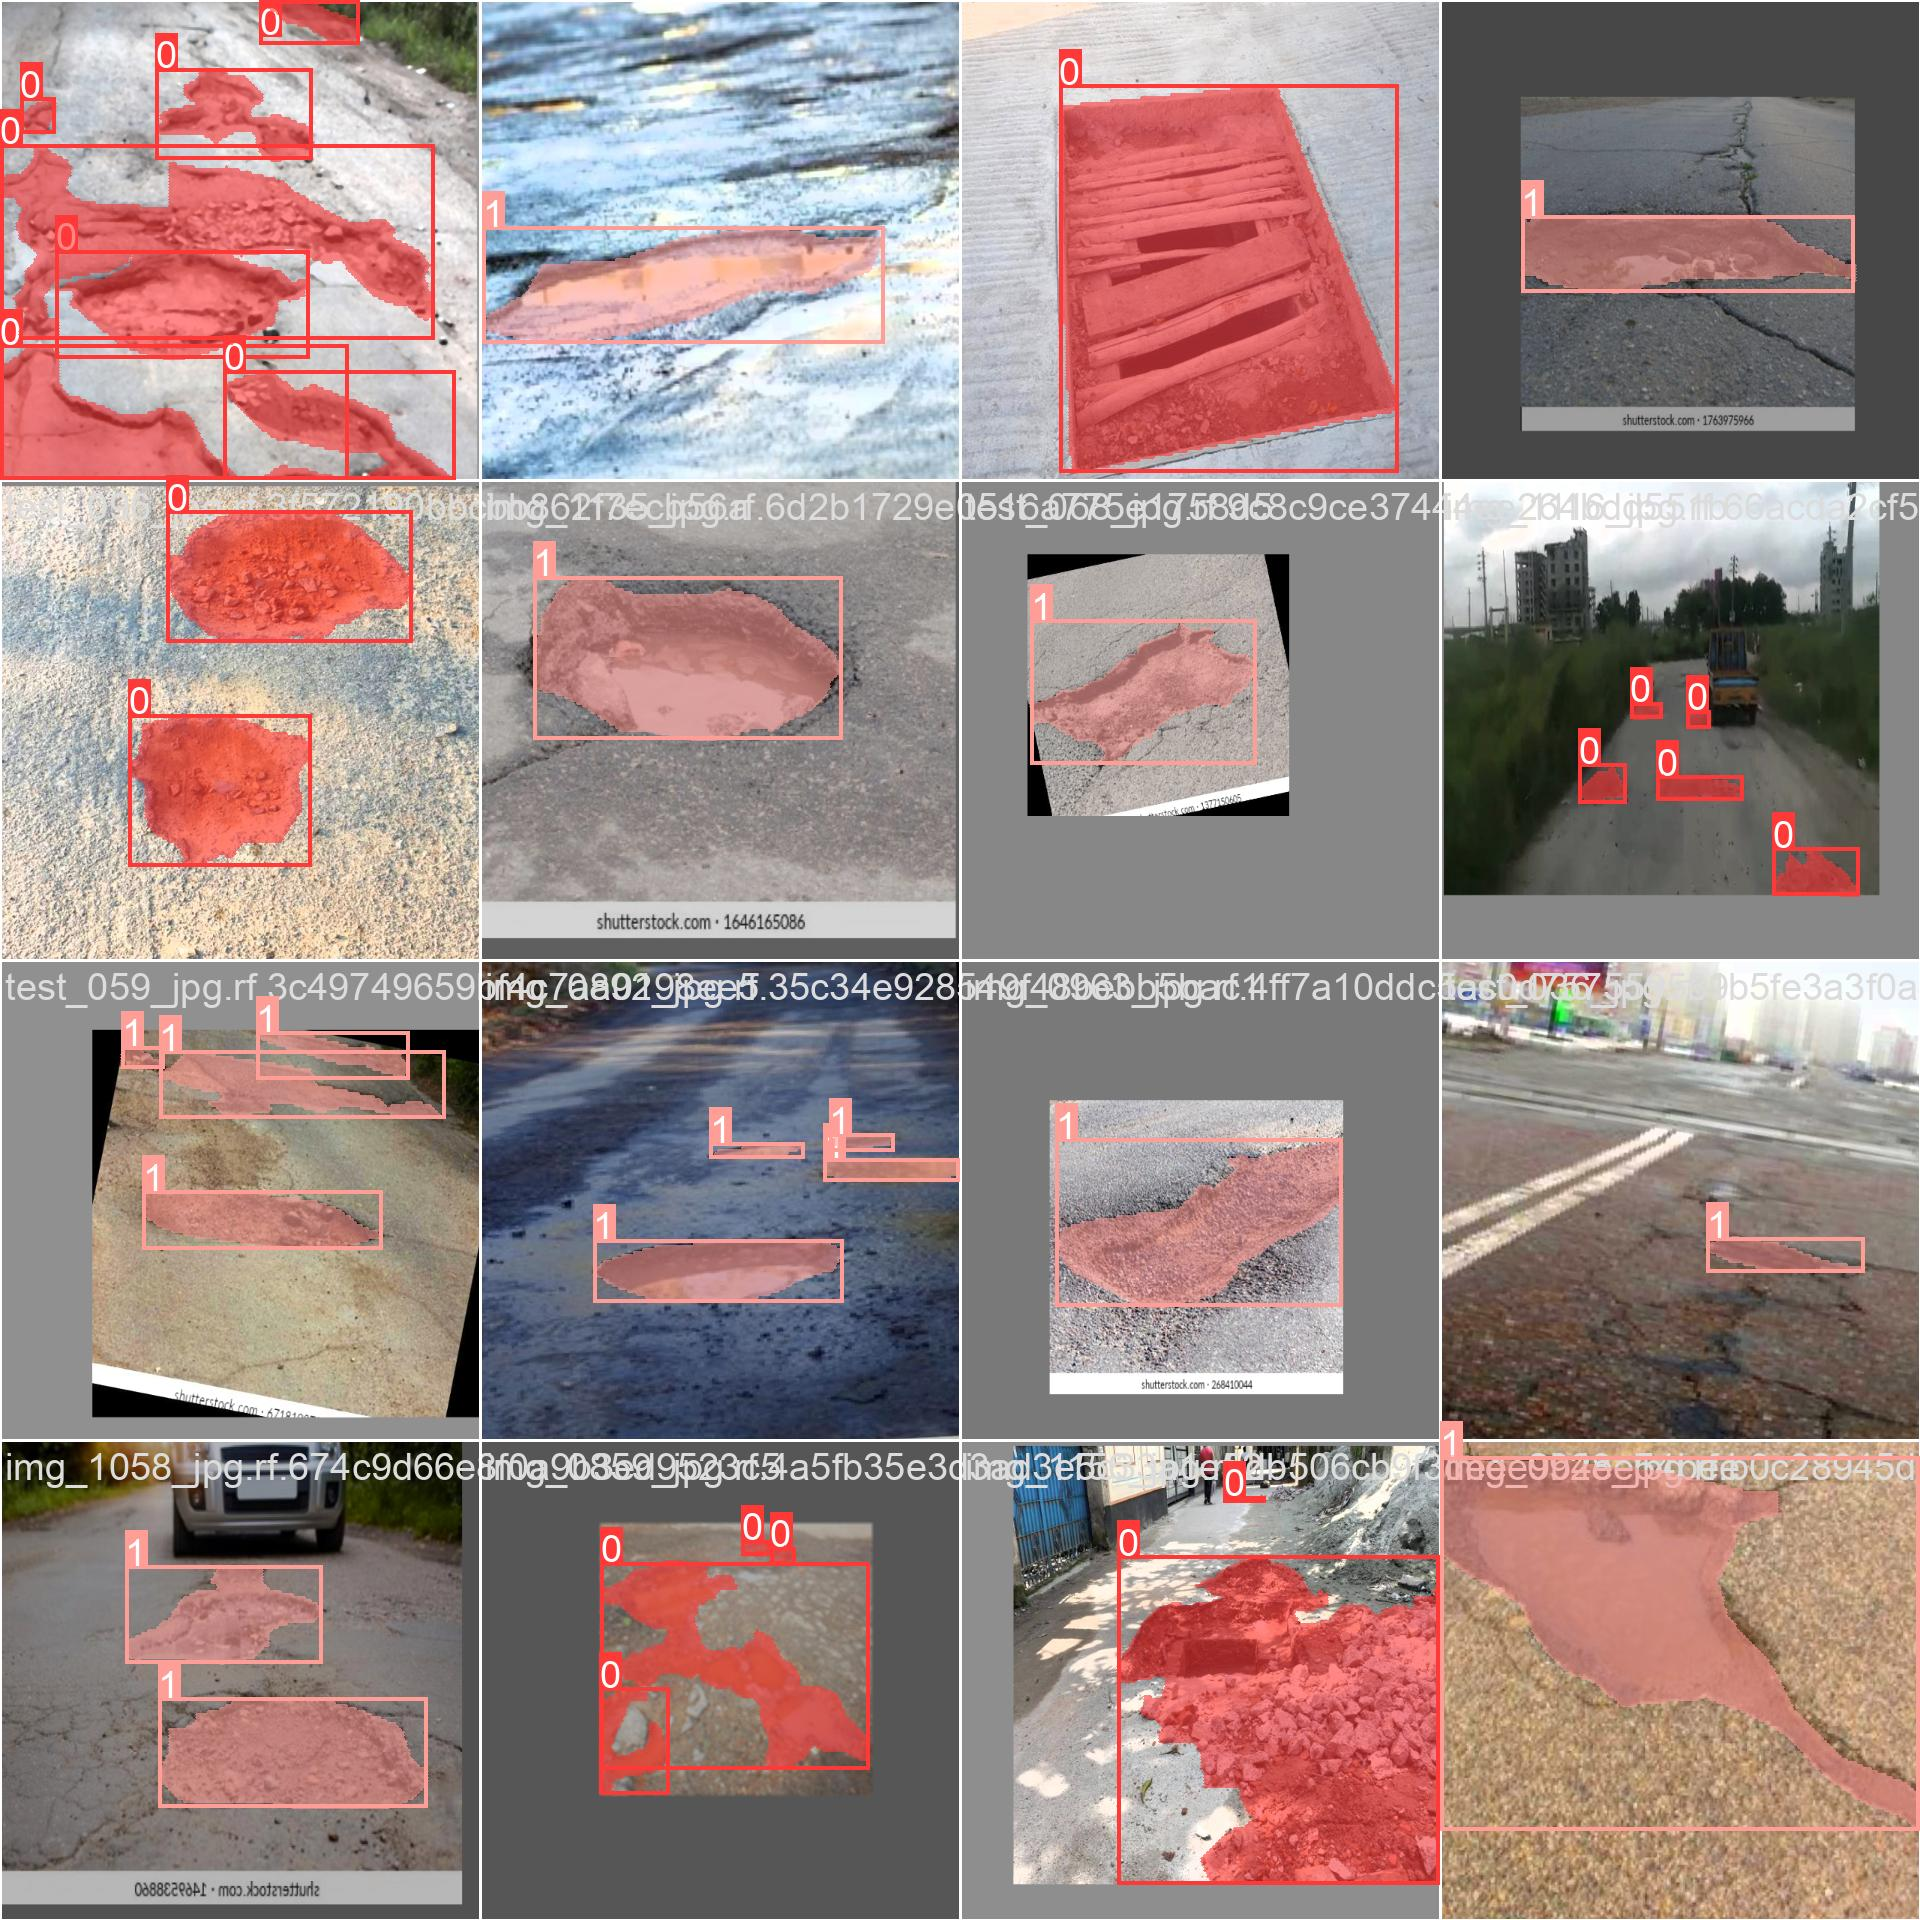
\includegraphics[width=15cm]{figs/cap6/train_results.jpg}
	\end{center}
	\caption{Demostración del modelo funcionando}
	\label{fig:trainex}
\end{figure}

Una vez demostrado que el modelo es capaz de detectar bien los baches, es el momento de convertir ese modelo para que fuera capaz de trabajar dentro de la RPi 4 y Google Coral. Gracias a este video\footnote{\url{https://www.youtube.com/watch?v=w4yHORvDBw0}}, se pudo conseguir realizar este Jupyter notebook\footnote{\url{https://colab.research.google.com/drive/1XU2ONX5Mq2zNWlZu3hmNIylqbto5hGfm?usp=sharing}} que convierte el modelo entrenado a un formato edgetpu de 192x192 imágenes, para que el dispositivo Google Coral pueda operar con él, llamado \textit{bestv2\_full\_integer\_quant\_edgetpu.tflite}\footnote{\url{https://github.com/RoboticsURJC/tfg-jlopez/blob/main/code/ros2/src/pibotj_rr/custom_model_lite/bestv2_full_integer_quant_edgetpu.tflite}}.

\subsubsection{Valores obtenidos del modelo}
\label{subsec:valoresmodelotflite}

Del presente modelo se pueden obtener los detalles de entrada y de salida del modelo, una vez se ha cargado. De entrada podemos encontrar los siguientes valores: 

\begin{verbatim}
	[{'name': 'serving_default_images:0', 'index': 0, 'shape': 
		array([  1, 192, 192,   3], dtype=int32), 'shape_signature': 
		array([  1, 192, 192,   3], dtype=int32), 'dtype': <class 'numpy.int8'>, 
		'quantization': (0.01865844801068306, -14), 'quantization_parameters': 
		{'scales': array([0.01865845], dtype=float32), 
		'zero_points': array([-14], dtype=int32), 'quantized_dimension': 0}, 
		'sparsity_parameters': {}}]
\end{verbatim}

Este tensor define la entrada para un modelo cuantizado que toma imágenes RGB de tamaño 192x192, en formato entero de 8 bits (int8). La cuantización utiliza una escala de 0.0187 y un punto cero de -14, mapeando los valores al rango del tensor int8, lo que ayuda a mejorar la eficiencia del modelo. Por otro lado, de salida podemos encontrar los siguientes valores: 

\begin{verbatim}
	[{'name': 'PartitionedCall:0', 'index': 2, 'shape': 
		array([  1,  38, 756], dtype=int32), 'shape_signature': 
		array([  1,  38, 756], dtype=int32), 'dtype': <class 'numpy.int8'>,
		'quantization': (0.017339961603283882, 12), 'quantization_parameters':
		{'scales': array([0.01733996], dtype=float32), 
		'zero_points': array([12], dtype=int32), 'quantized_dimension': 0},
	  	'sparsity_parameters': {}},
	{'name': 'PartitionedCall:1', 'index': 1, 'shape': 
		array([ 1, 48, 48, 32], dtype=int32), 'shape_signature': 
		array([ 1, 48, 48, 32], dtype=int32), 'dtype': <class 'numpy.int8'>, 
		'quantization': (0.020256992429494858, -114), 'quantization_parameters': 
		{'scales': array([0.02025699], dtype=float32), 
		'zero_points': array([-114], dtype=int32), 'quantized_dimension': 0},
		'sparsity_parameters': {}}]
		
\end{verbatim}


Estos son dos tensores de salida en un modelo cuantizado. El primer tensor (PartitionedCall:0) tiene forma [1, 38, 756], y el segundo tensor (PartitionedCall:1) tiene forma [1, 48, 48, 32]. Ambos utilizan el formato int8 y aplican parámetros de cuantización específicos que ajustan el rango de valores, optimizando el modelo para dispositivos de bajo consumo. De ambos tensores el que nos interesa es el segundo y es debido a su forma. Posee 32 canales y para este proyecto únicamente nos interesan los canales 0 y 1 como muestra la Figura \ref{fig:trainex}.

\subsubsection{Aplicación del modelo}
\label{subsec:aplicacionmodelo}

Una vez se conocen las características que posee el modelo, es necesario extraer la información y convertirla en el formato adecuado para poder operar con ella (Código \ref{cod:codeconvert})

\begin{code}[h]
	\begin{lstlisting}[language=Python]
		# Redimensionar la imagen a las dimensiones requeridas por el modelo
		input_shape = self.input_details[0]['shape']
		height, width = input_shape[1], input_shape[2]
		resized_frame = cv2.resize(frame, (width, height))
		
		# Convertir la imagen a formato adecuado
		input_data = np.expand_dims(resized_frame, axis=0).astype(np.float32)
		# Normalizacion 
		input_data = (input_data - 127.5) / 127.5 
		
		# Convertir la imagen a int8
		scale, zero_point = self.input_details[0]['quantization']
		input_data = (input_data / scale + zero_point).astype(np.int8)
		
		# Establecer el tensor de entrada y realizar la inferencia
		self.interpreter.set_tensor(self.input_details[0]['index'], input_data)
		self.interpreter.invoke()
		
		# Saca informacion del tensor de salida 2 que tiene forma [1, 48, 48, 32] 
		output_data1 = self.interpreter.get_tensor(self.output_details[1]['index'])
		# elimina la dimensipn del batch (el primer valor del array)
		prediction1 = np.squeeze(output_data1)
		
		# Descuantificar la mascara de baches mirando el canal 0
		pothole_mask_class0 = (prediction1[:, :, 0].astype(np.float32) - zero_point) * scale
		# Descuantificar la mascara de baches mirando el canal 1
		pothole_mask_class1 = (prediction1[:, :, 1].astype(np.float32) - zero_point) * scale
	\end{lstlisting}
	\caption[Cómo convertir los datos del modelo a un formato adecuado]{Cómo convertir los datos del modelo a un formato adecuado}
	\label{cod:codeconvert}
\end{code}

Los valores de \verb|pothole_mask_class0| y \verb|pothole_mask_class1| ya se pueden tratar y establecer una umbralizacización de 0.6 para considerar dichos valores si han detectado bache o no. Sin embargo, los valores de \verb|pothole_mask_class0| y \verb|pothole_mask_class1| eran muy inestables y se consideró la técnica de \ac{EMA} (Ecuación \ref{ec:ema}) para que no fluctuasen tanto los valores y darle más peso a las medidas más recientes. Esta técnica es común en análisis técnico, como se describe en \cite{6708545}, pero se decidió incluir en ese proyecto ya que satisfacía las necesidades buscadas y por su liviana carga computacional.

\begin{myequation}[h]
	\begin{equation}
		S_t = \alpha \cdot Y_t + (1 - \alpha) \cdot S_{t-1}
		\nonumber
		\label{ec:ema}
	\end{equation}
	\caption[Fórmula de la media móvil exponencial]{Fórmula de la media móvil exponencial}
\end{myequation} 

Siendo $\alpha$  el valor de grado de disminución de ponderación, $Y_t$ el valor actual en tiempo t, $S_t$ es el valor de \acs{EMA} en tiempo t y $S_{t-1}$ es el valor de \acs{EMA} en tiempo t-1.
 
\subsubsection{Obtención del contorno y coordenadas}
\label{subsec:contornoycoordenadas}

Después de saber si en una imagen había bache o no, se consideraría bache si la detección ocurre durante 3 segundos sin interrupciones. Una vez pasado ese tiempo, había que publicar los píxeles asociados a ese contorno. 

Para conseguir los píxeles, se toma la máscara binarizada usando el umbral definido previamente de 0.6. De esa forma, es posible encontrar los píxeles del contorno más grande de la máscara pero, esos píxeles están en base a las dimensiones de la máscara que es de 48x48 píxeles; así que, es necesario aplicar un factor de escala para que los píxeles estén en base a la imagen que es de 192x192 píxeles. Se puede ver un resultado final del contorno detectado en la Figura \ref{fig:contornobache}.
  

\begin{figure}[ht!]
	\centering
	\begin{minipage}{0.4\linewidth}
		\centering
		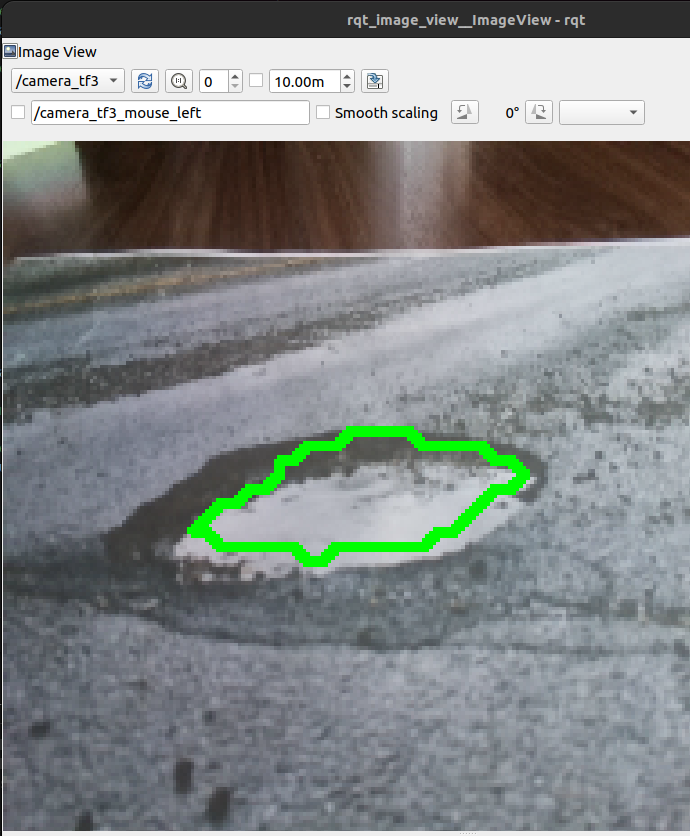
\includegraphics[width=\linewidth]{figs/cap6/contornobache1.png}
	\end{minipage}
	\hspace{2 cm}
	\begin{minipage}{0.4\linewidth}
		\centering
		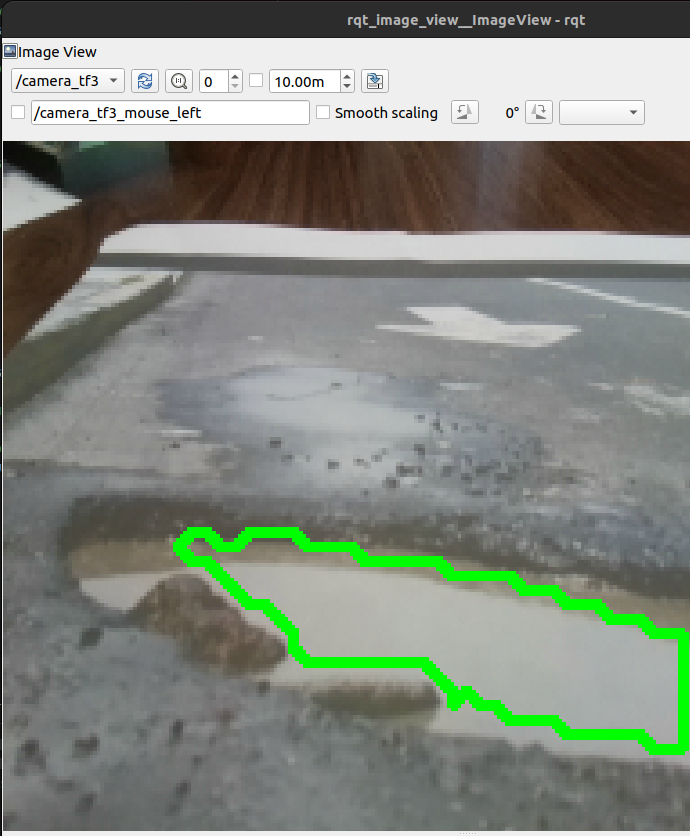
\includegraphics[width=\linewidth]{figs/cap6/contornobache2.png}
	\end{minipage}
	\caption{Contorno del baches detectados}
	\label{fig:contornobache}
\end{figure}

\subsection{Cámara pinhole}
\label{subsec:softwarehsuelo}

Extraer información de la cámara no es fácil y por ello se decidió simplificar la cámara definiéndola como una cámara \textit{pinhole}, o también conocida como una cámara estenopeica. El modelo \textit{pinhole} describe una cámara (sin lente) y con una pequeña apertura. Los rayos de luz atraviesan la apertura y proyectan una versión invertida de lo que se capta en el fondo de la cámara (o el plano de la imagen) (Figura \ref{fig:pinhole}).

 \begin{figure} [h!]
	\begin{center}
		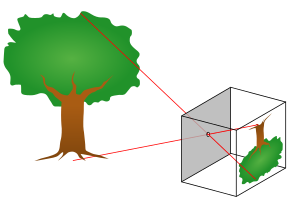
\includegraphics[width=8cm]{figs/cap6/pinhole.png}
	\end{center}
	\caption{Funcionamiento de una cámara esteneopeica $^{\ref{note:enlace124}}$}
	\label{fig:pinhole}
\end{figure}

% Definir la primera nota al pie con el número 124
\setcounter{footnote}{124} % Reiniciar la numeración de notas al pie
\footnotetext[\value{footnote}]{\url{https://es.wikipedia.org/wiki/C\%C3\%A1mara_estenopeica}\label{note:enlace124}}


Este modelo explica cómo se realiza la proyección de un punto en el espacio tridimensional hacia el plano bidimensional de una imagen. En otras palabras, el modelo de cámara define una fórmula matemática que, a partir de las coordenadas de un punto en el espacio 3D, con referencia a la cámara, permite calcular las coordenadas en las que ese punto aparecería en una fotografía. Un resumen de fórmulas matemáticas aparecen en la Figura \ref{fig:pinholeformula}.

 \begin{figure} [h!]
	\begin{center}
		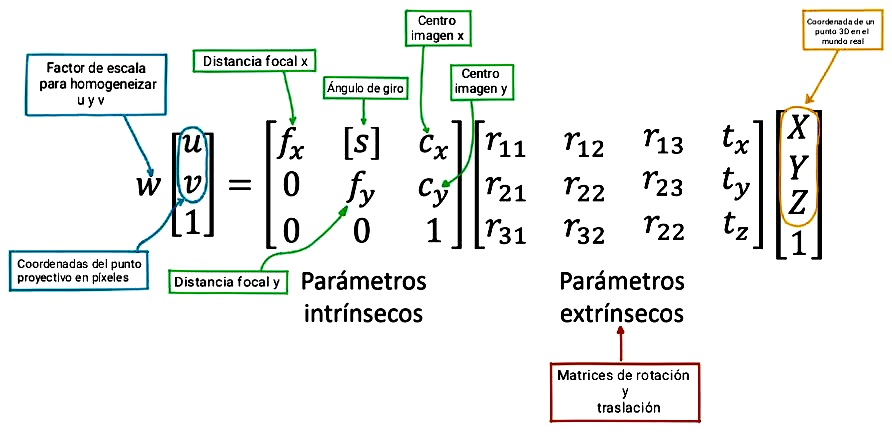
\includegraphics[width=15cm]{figs/cap6/esquema_pinhole_matrices.jpg}
	\end{center}
	\caption{Relación de fórmulas del modelo pinhole}
	\label{fig:pinholeformula}
\end{figure}
  
En la Figura \ref{fig:pinholeformula} se pueden ver los pámetros intrínsecos y extrínsecos que son tomados de la calibración de la cámara, descritos en la Sección \ref{subsec:configcamara}. Dicha calibración se realizó sobre imágenes de 640x480 y los píxeles del contorno del bache está en base de imágenes de 192x192, por lo que era necesario aplicar otro factor de conversión. 

Una vez se conoce cómo funciona el modelo pinhole, es importante destacar que para poder convertir los píxeles del mundo 2D al mundo real, hay que tener en cuenta que hay tres sistemas de coordenadas diferentes como muestra la Figura \ref{fig:siscoordenadas} que ha sido obtenida del artículo \cite{unknown} y que el modelo pinhole únicamente es capaz de convertir del sistema de coordenadas del mundo real al sistema de coordenadas de la cámara, algo a tener en cuenta.  

 \begin{figure} [h!]
	\begin{center}
		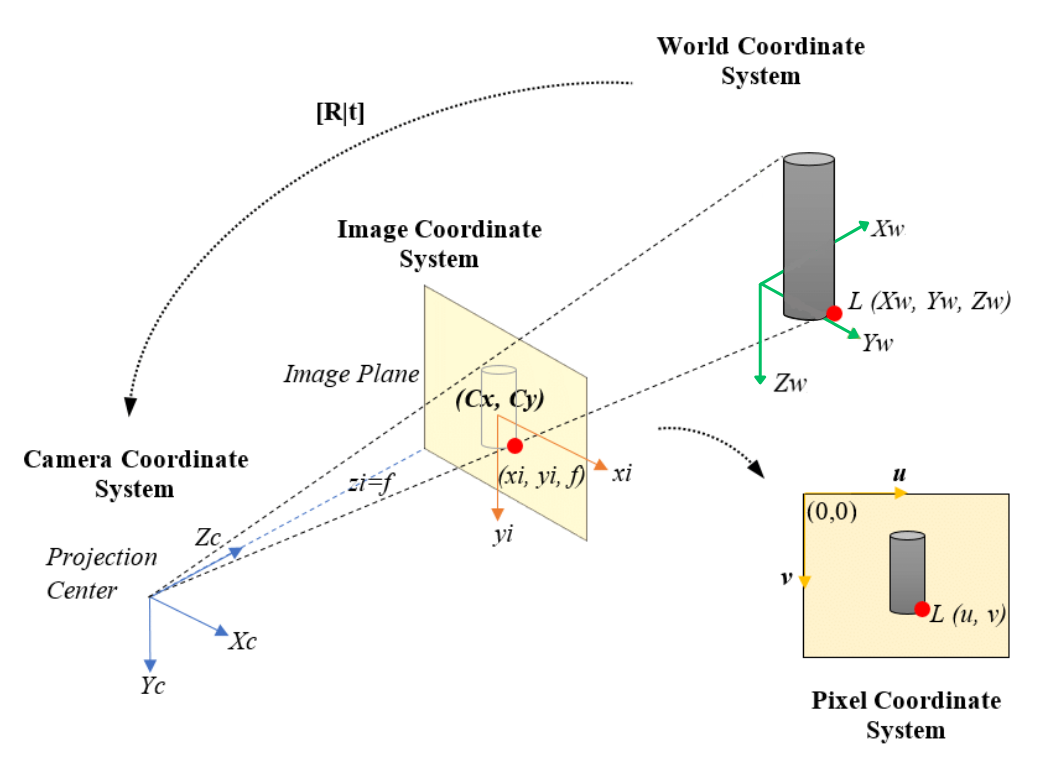
\includegraphics[width=15cm]{figs/cap6/pinholecoordinates.png}
	\end{center}
	\caption{Sistemas de coordenadas}
	\label{fig:siscoordenadas}
\end{figure}

Otro dato importante a tener en cuenta es que solo disponemos de una cámara, y por tanto, el sistema no puede encontrar el punto 3D asociado en una imagen debido a que cada punto de la línea OX proyecta al mismo píxel en el plano imagen; se pierde el valor de la profundidad (eje Z). Además, al hacer la conversión entre los distintos sistemas de coordenadas del modelo \textit{pinhole}, el valor de profundidad (de Z) también se pierde. Es por todo lo dicho anteriormente que hay que emplear la hipótesis suelo. 

La hipótesis suelo (Figura \ref{fig:hipotesissuelo} tomada del artículo \cite{vega19d}) supone que todos los objetos del mundo en 3D están pegados al suelo, por lo tanto, asumiendo que Z = 0, nos permitirá estimar la conversión de 2D a 3D con una sola cámara.  

 \begin{figure} [h!]
	\begin{center}
		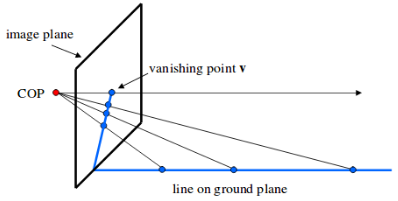
\includegraphics[width=9cm]{figs/cap6/hipotesissuelo.png}
	\end{center}
	\caption{La hipótesis suelo asume que todos los objetos están en el suelo}
	\label{fig:hipotesissuelo}
\end{figure}

Para conseguir la solución a este problema la tomamos del artículo \cite{vega19d}, donde los autores nos presentan un sistema de visión de código abierto que simplifica el uso de cámaras en la robótica educativa. En él se detallan todos los pasos que se han explicado previamente y el código asociado con la obtención de los píxeles en coordenadas del mundo en 3D, se encuentra definido en \verb|camera_pinholev2_node.py|\footnote{\url{https://github.com/RoboticsURJC/tfg-jlopez/blob/main/code/ros2/src/pibotj_rr/pibotj_rr/camera_pinholev2_node.py}}.

\subsection{Algoritmo de la lazada}
\label{subsec:softwareshoelace}

Para calcular el área de las coordenadas del mundo real, se ha obtado por seguir el algoritmo de la lazada\footnote{\url{https://es.wikipedia.org/wiki/F\%C3\%B3rmula_del_\%C3\%A1rea_de_Gauss}} o también conocido como el área de Gauss. Este algoritmo matemático es usado para calcular el área de un polígono simple cuyos vértices están descritos como pares de coordenadas en el plano. Tiene múltiples aplicaciones en agrimensura y topografía.

El nombre de este algoritmo es debido al constante cruce de productos de las coordenadas, que simula atarse los cordones, como muestra la \ref{ec:shoelace}.
\begin{myequation}[h]
	\begin{equation}
		A = \frac{1}{2}\abs{\sum_{i=1}^{n-1}x_i y_{i+1} + x_n y_1 - \sum_{i=1}^{n-1}x_{i+1} y_{i} - x_1 y_n}
		\nonumber
		\label{ec:shoelace}
	\end{equation}
	\caption[Fórmula del algoritmo de la lazada]{Fórmula del algoritmo de la lazada}
\end{myequation} 

Donde A es el área del polígono, n es el número de lados del polígono y $(x_i, y_i)$ , i = 1,2,...,n son los vértices del polígono de forma alternativa.

Un ejemplo que ilustra estre proceso y demuestra que se cumple el algoritmo de la lazada con respecto a la fórmula usada para calcular el área de un rectángulo, se puede apreciar en la Figura \ref{fig:demoshoelace}.

 \begin{figure} [h!]
	\begin{center}
		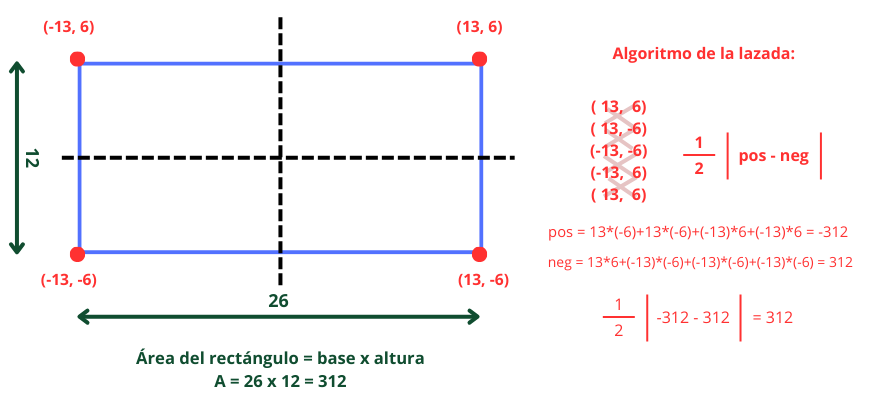
\includegraphics[width=15cm]{figs/cap6/demoshoelace.png}
	\end{center}
	\caption{Demostración del algoritmo de la lazada}
	\label{fig:demoshoelace}
\end{figure}


Este algoritmo aparece aplicado una vez que se ha convertido las coordenadas al sistema del mundo real en \verb|camera_pinholev2_node.py|\footnote{\url{https://github.com/RoboticsURJC/tfg-jlopez/blob/main/code/ros2/src/pibotj_rr/pibotj_rr/camera_pinholev2_node.py}}.


\subsection{Interfaz Web}
\label{subsec:softwareweb}
La forma que se decidió usar la \ac{HRI} para poder cumplir con el objetivo principal descrito en la Sección \ref{sec:descripcion}, fue a través de una interfaz web. Dicha interfaz web, ha sido creada gracias a las herramientas descritas en la Sección \ref{subsec:interfazweb}. \verb|Rosbridge_server| permite a las páginas web (que actúan como clientes) comunicarse con el servidor (que en este caso se inicializa en PiBotJ). Para acceder como cliente, en una ventana de un navegador hay que escribir \verb|http://<ip de PiBotJ>:8000/index.html|, sustituyendo \verb|<ip de PiBotJ>| por la IP obtenida al conectarse PiBotJ a la red.
 
Una vez habilitada esa comunicación, ya se podía apreciar la página web\footnote{\url{https://github.com/RoboticsURJC/tfg-jlopez/blob/main/code/ros2/index.html}} (Figura \ref{fig:interfazweb}). Se decidió incluir un mapa, usando OpenStreetMaps, en el que apareciese un marcador que tiene asociado el valor de área/volumen por cada bache detectado. Por otro lado, se decidió incluir una botonera para poder ser capaz de controlar el movimiento de las ruedas de PiBotJ cuando se quiera usar el modo teleoperado. Dicha botonera se conforma de cuatro botones que publican los distintos movimientos al robot, y cuando se deja de pulsar, el robot se para.

% PENSAR SI INCLUIR VIDEO DEL MODO TELEOPERADO O NO O UN VIDEO DONDE SE MUEVA ÚNICAMENTE LAS RUEDAS.

\begin{figure} [h!]
	\begin{center}
		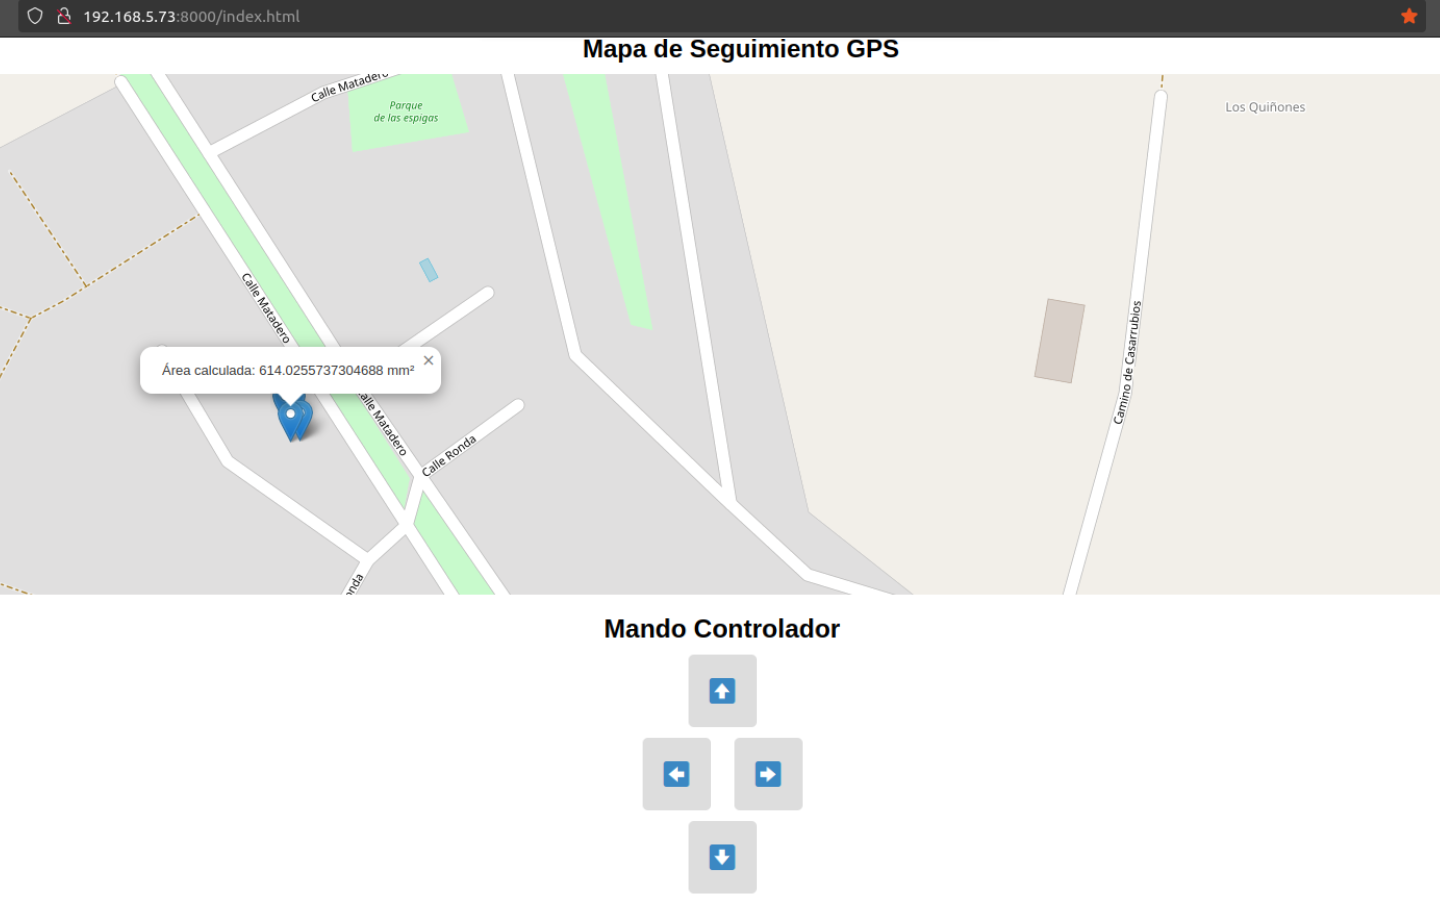
\includegraphics[width=15cm]{figs/cap6/interfazweb.png}
	\end{center}
	\caption{Interfaz web}
	\label{fig:interfazweb}
\end{figure}


\subsection{Autónomo}
\label{subsec:autonomo}
PiBotJ ya se ha visto que se puede controlar de forma teleoperada, usando la botonera definida en la Sección \ref{subsec:softwareweb} pero, para tener otra alternativa con respecto a la navegación de PiBotJ, se ha decidido implementar una lógica para que su movimiento sea autónomo. 

Lo ideal para este caso es que PiBotJ fuera capaz de navegar  autónomamente por carreteras pero debido a la imposibilidad de probarlo en ese entorno, se decidió hacer una recreación de una carretera real\footnote{\url{https://www.totalmentereflejante.com/medidas-rayas-de-carretera/}} a escala 769:10000 sobre una cartulina negra. En la Figura \ref{fig:medidascarretera} (izquierda) se muestran las medidas reales y en la Figura \ref{fig:medidascarretera} (derecha) se muestra las medidas definidas. El resultado final aparece en la Figura \ref{fig:carreteracartulina}.

\begin{figure}[ht!]
	\centering
	\begin{minipage}{0.45\linewidth}
		\centering
		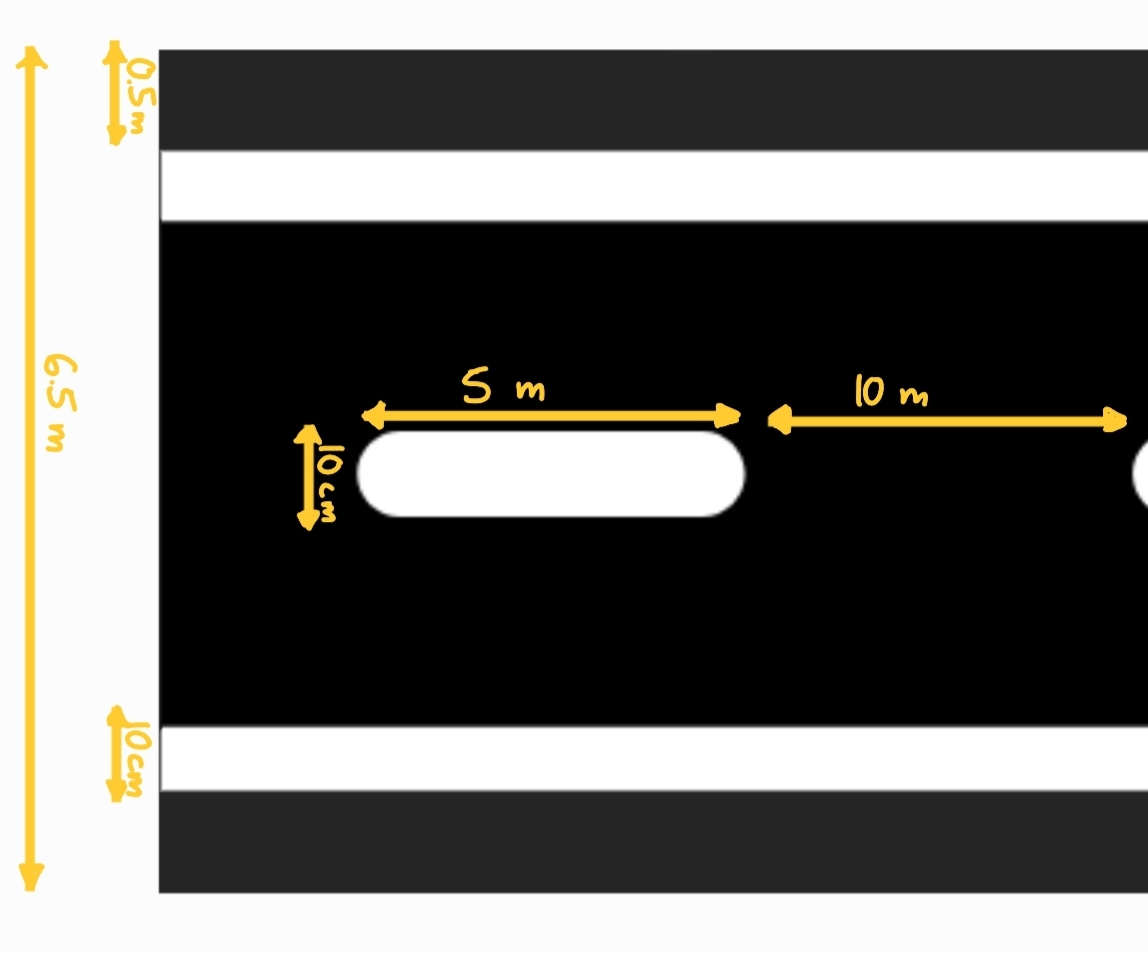
\includegraphics[width=\linewidth]{figs/cap6/medidas_reales.jpg}
		\caption*{\centering Medidas reales} 
	\end{minipage}
	\hspace{1 cm}
	\begin{minipage}{0.45\linewidth}
		\centering
		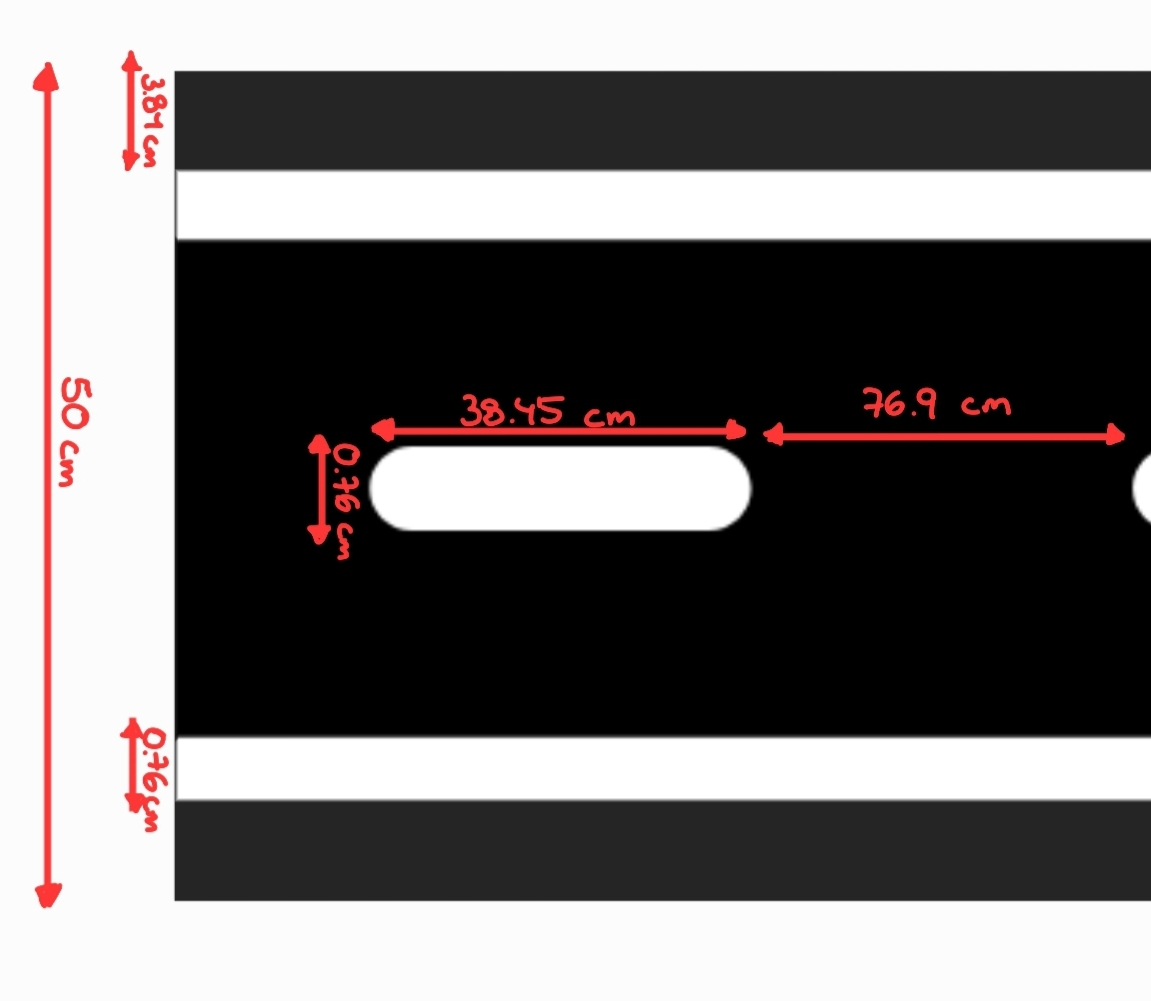
\includegraphics[width=\linewidth]{figs/cap6/medidas_ficticias.jpg}
		\caption*{\centering Medidas para la cartulina}
	\end{minipage}
	\caption{Conversión de medidas de la carretera}
	\label{fig:medidascarretera}
\end{figure}

 \begin{figure} [h!]
	\begin{center}
		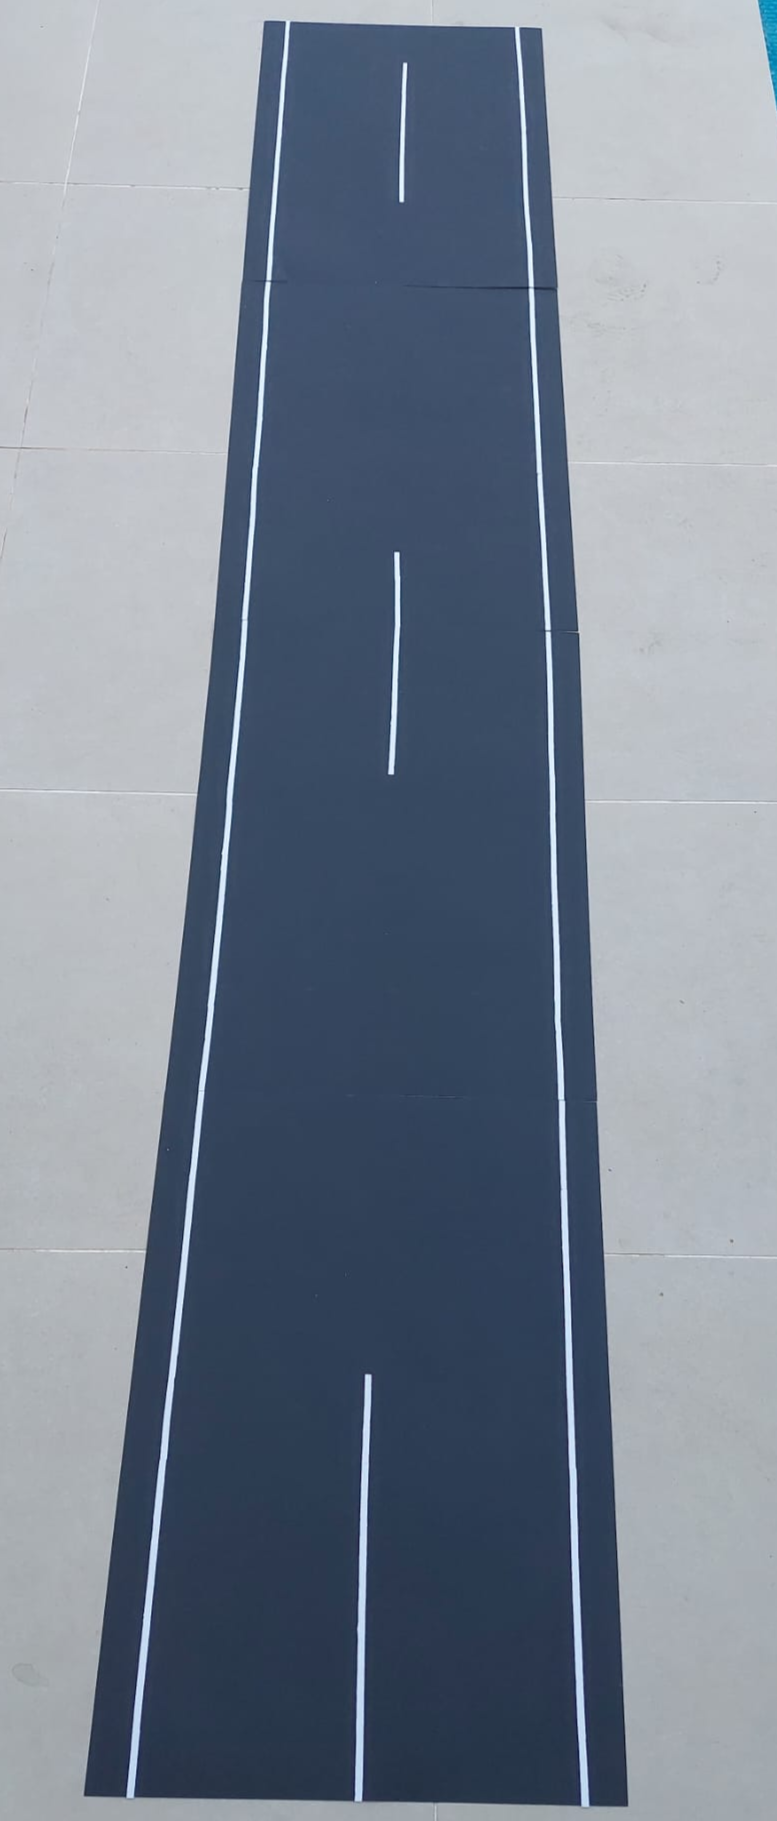
\includegraphics[width=6cm, height=6cm]{figs/cap6/carretera.png}
	\end{center}
	\caption{Carretera creada en cartulina}
	\label{fig:carreteracartulina}
\end{figure}

Una vez definido el entorno donde se iba a trabajar, era el momento de definir la lógica a usar y se decidió unir un algoritmo de detección de líneas junto a la técnica de navegación local conocida como \ac{VFF}. 

\subsubsection{Detección de líneas}
\label{subsubsec:softwaredl}

Es importante a tener en cuenta que este algoritmo se va a ejecutar únicamente cuando no haya bache en el entorno controlado. Para conseguirlo, es necesario procesar la imagen en escala de grises para detectar los contornos de las líneas, usando una umbralización adaptativa para destacar los bordes y una operación de apertura morfológica para eliminar pequeños puntos blancos que representan ruido en la imagen binaria (Código \ref{cod:dl}). El resultado final queda reflejado en la Figura \ref{fig:camaradlines} y el código está plasmado en \verb|camera_dl_node.py|\footnote{\url{https://github.com/RoboticsURJC/tfg-jlopez/blob/main/code/ros2/src/pibotj_rr/pibotj_rr/camera_dl_node.py}}.


\begin{code}[h]
	\begin{lstlisting}[language=Python]
	# Convierte la imagen a escala de grises
	gray = cv2.cvtColor(resized_frame, cv2.COLOR_BGR2GRAY)
	# Aplica un umbral para destacar los bordes
	th1 = cv2.adaptiveThreshold(gray,255,cv2.ADAPTIVE_THRESH_MEAN_C, cv2.THRESH_BINARY,23,-50)
		
	# Elimina ruido
	kernel = np.ones((3, 3), np.uint8) 
	opened_th1 = cv2.morphologyEx(th1, cv2.MORPH_OPEN, kernel)
	\end{lstlisting}
	\caption[Filtro para obtener las líneas blancas]{Filtro para obtener las líneas blancas}
	\label{cod:dl}
\end{code}


 \begin{figure} [h!]
	\begin{center}
		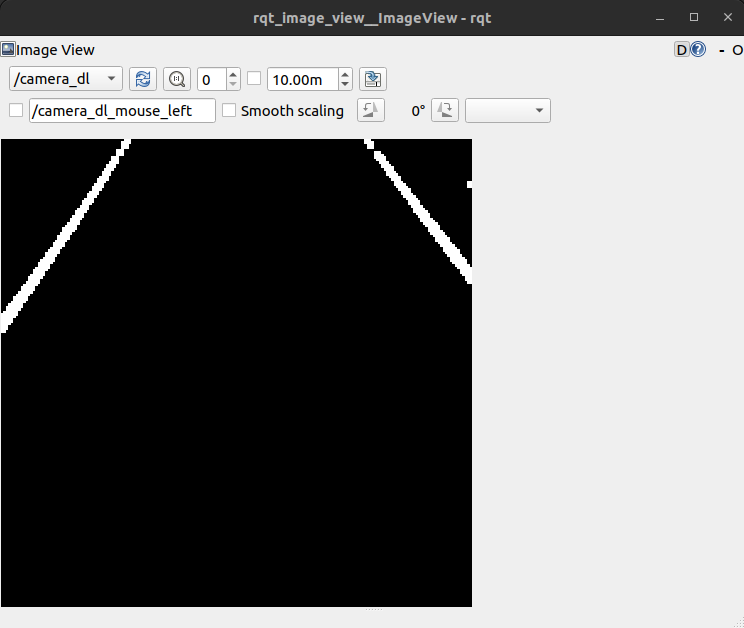
\includegraphics[width=9cm]{figs/cap6/camaradlines.png}
	\end{center}
	\caption{Filtro resultante aplicado para la detección de líneas}
	\label{fig:camaradlines}
\end{figure}


%Incluir una imagen detectando las líneas. Incluir un video detectando las lineas
En la Figura \ref{fig:dlines} se puede ver los distintos tipos de situaciones a las que se enfrenta PiBotJ cuando detecta líneas y dependiendo de la situación, PiBotJ reaccionaría de una forma u otra. Cuando detecta las dos líneas, PiBotJ sigue recto mientras que si detecta únicamente una línea, deberá avanzar hacia adelante y si dicha línea no se encuentra en el centro de la imagen, PiBotJ giraría hasta que se situase en el centro. Por otro lado, si no detecta líneas avanzaría recto durante 3 segundos y empezaría a girar.

 \begin{figure} [h!]
	\begin{center}
		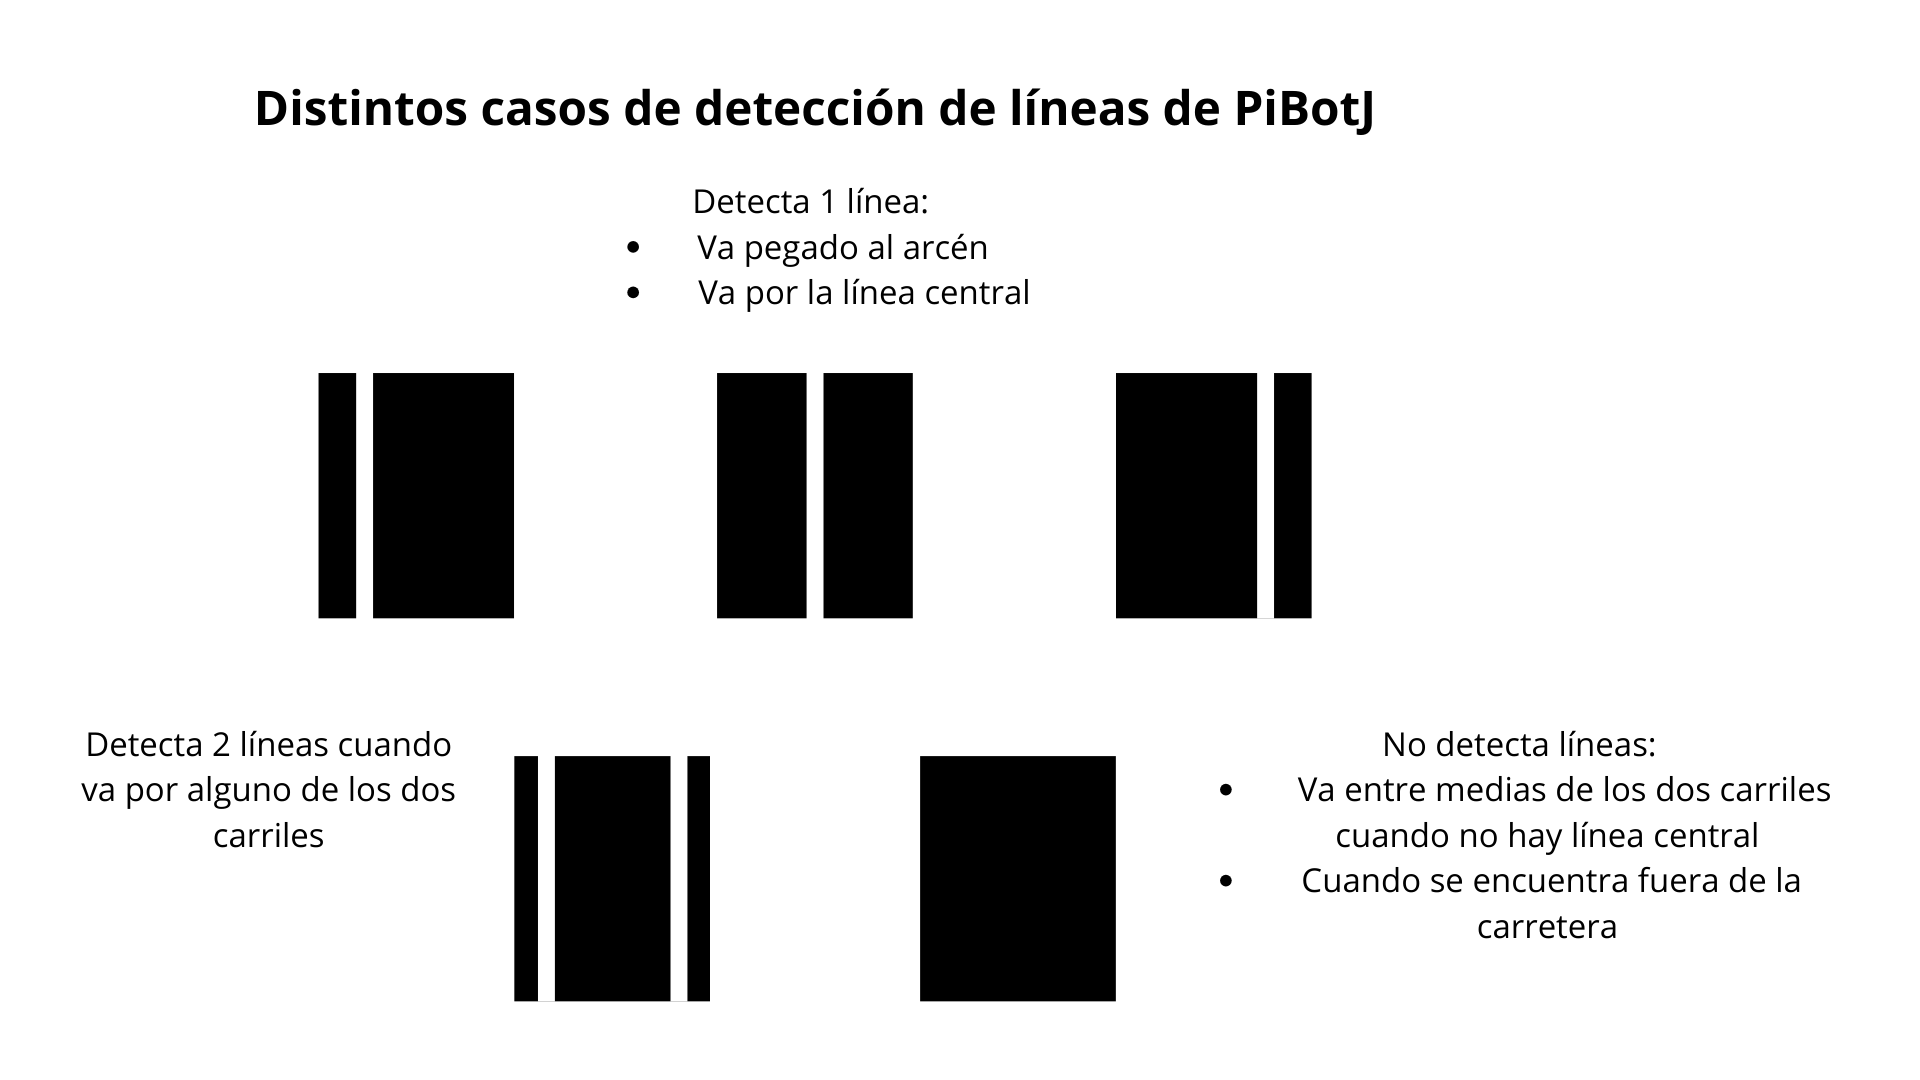
\includegraphics[width=15cm]{figs/cap6/casosdlines.png}
	\end{center}
	\caption{Distintos casos de la detección de líneas}
	\label{fig:dlines}
\end{figure}

\subsubsection{Virtual Force Field}
\label{subsubsec:vff}

Es un método de navegación local para que un robot autónomo evite obstáculos en su entorno. Este método se compone de una fuerza repulsiva para evitar el obstáculo y de una fuerza atractiva para alcanzar el destino objetivo\footnote{\url{https://robmovjuloau2022.blogspot.com/2022/11/task-3-local-navigation-with-vff.html}}. Estas fuerzas se suman vectorialmente para obtener una fuerza resultante, que indica la dirección y velocidad de movimiento del robot. Esta fuerza resultante se puede calcular siguiendo la Ecuacion \ref{ec:vff}.

\begin{myequation}[h]
	\begin{equation}
		F_{resultante} = \alpha \cdot F_{atractiva} + \beta \cdot F_{repulsiva}
		\nonumber
		\label{ec:vff}
	\end{equation}
	\caption[Ecuación de VFF]{Ecuación de VFF}
\end{myequation} 

El robot se mueve en la dirección de la fuerza resultante, ajustando su trayectoria en tiempo real según las posiciones del obstáculo y el objetivo. En este caso, se decidió fijar como objetivo, un punto siempre hacia adelante y como repulsión, el punto más cercano detectado del contorno al robot, en coordenadas del mundo real, y aplicar la fuerza repulsiva respecto a él. La Figura \ref{fig:vfffuerzas} muestra la dirección de las distintas fuerzas. Todo está documentado en \verb|camera_vff_node.py|\footnote{\url{https://github.com/RoboticsURJC/tfg-jlopez/blob/main/code/ros2/src/pibotj_rr/pibotj_rr/camera_vff_node.py}}.


 \begin{figure} [h!]
	\begin{center}
		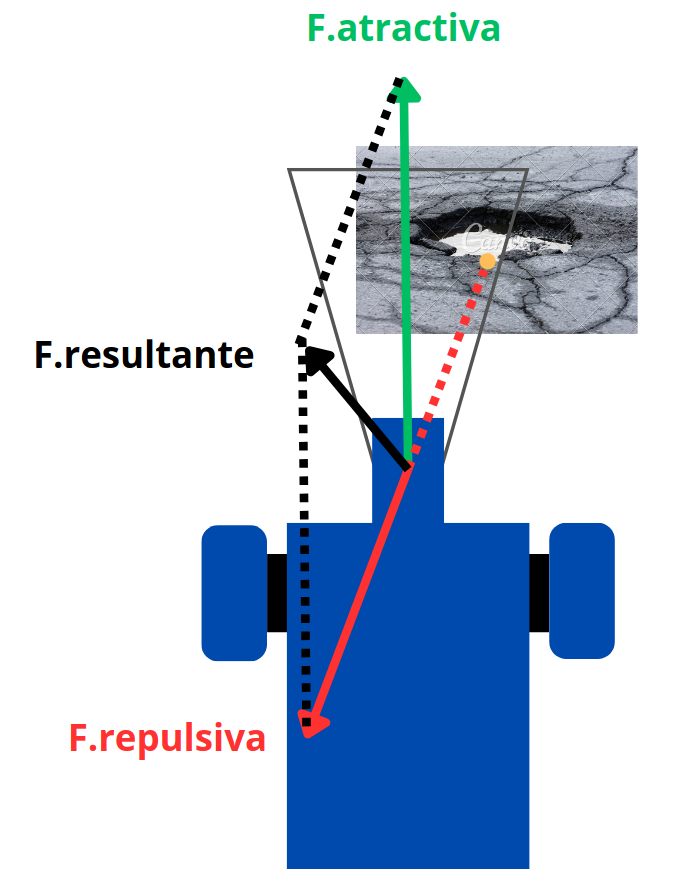
\includegraphics[width=10cm]{figs/cap6/vff.png}
	\end{center}
	\caption{Diagrama de fuerzas del algoritmo VFF}
	\label{fig:vfffuerzas}
\end{figure}

